%% Copyright (C) 2011, Andrea Cimino, All Rights Reserved.
%% This file is distributed under the terms of the Creative Commons
%% Licence Non-Commercial Share-Alike license


%% Useful stuff for separate compilation.
\ifx\ismaindoc\undefined
\providecommand{\inbpdocument}{
 \documentclass[11pt,a4paper,twoside,titlepage]{scrbook}
%%%%%%%%%%%%%%%%%%%%%%%%%%%%%%%%
%%%%%%%%%%% PACKAGES %%%%%%%%%%%
%%%%%%%%%%%%%%%%%%%%%%%%%%%%%%%%
% encoding
\usepackage[utf8x]{inputenc}
\usepackage[italian]{babel} % babel (suddivisione parole in sillabe)

\usepackage{amsfonts} % matematica
\usepackage{amsmath} % matematica
\usepackage{amssymb} % simboli vari
\usepackage{calrsfs}
\usepackage{caption}
\usepackage{enumerate}
\usepackage{extarrows} % matematica
\usepackage{keyval}
\usepackage{manfnt} % Simboli curva
\usepackage{mathtools} % matematica
\usepackage{multirow} 
\usepackage[usenames, dvipsnames]{color} % colori con nome
\usepackage[pdftex]{graphicx}
\usepackage{epstopdf} % gestione file EPS
\usepackage{wrapfig} % per figure circondate da testo
\usepackage{framed}	% teoremi framed
\usepackage{fancyhdr} % header buffi
\usepackage[T1]{fontenc} % gestione hbox e vbox
\usepackage[a4paper]{geometry}
\usepackage{microtype} % gestione hbox e vbox
\usepackage[thref, amsthm, amsmath, framed, hyperref]{ntheorem} % teoremi (avanzata)
%% \usepackage{prooftree} % gestione prof-tree
\usepackage{rotating}
\usepackage{stmaryrd}
\usepackage{subfig}
\usepackage{syntax} % syntattic stuff
\usepackage{txfonts}
\usepackage{verbatim} % migliorie al verbatim
%\usepackage{hyperref}
%% \usepackage{qtree}
\usepackage{fancyvrb}
\usepackage{listings}
\usepackage{cancel}
\usepackage{tikz}

\usepackage{bbding} %% Icons

%%%%%%%%%%%%%%%%%%%%%%%%%%%%%%%%
%%%%%%%%%%% GEOMETRY %%%%%%%%%%%
%%%%%%%%%%%%%%%%%%%%%%%%%%%%%%%%
\geometry{verbose,tmargin=2cm,bmargin=2.5cm,lmargin=2.5cm,rmargin=2cm}
\parindent0ex %% Remove paragraph indenting

%%%%%%%%%%%%%%%%%%%%%%%%%%%%%%%%
%%%%%%%%%%% CODE ENV %%%%%%%%%%%
%%%%%%%%%%%%%%%%%%%%%%%%%%%%%%%%
% codice
\newcounter{count}
\setcounter{count}{0}
\newenvironment{code}[1]
{
\color{lightgray}\hrulefill\color{code}
\stepcounter{count} {\bf\small Listato di codice \arabic{count}: {#1} }
\verbatim
}
{
\endverbatim
\color{lightgray}\hrulefill
\color{black}
\\
}

% codice semplice
\newenvironment{simplecode}
{
\color{code} \tt
}
{
\rm
}

 % Notation issues

%% Proof trees.
%\input prooftree
\newcommand*{\nohyp}{\phantom{x}}

%% C++.
\newcommand*{\Cplusplus}{{C\nolinebreak[4]\hspace{-.05em}\raisebox{.4ex}
{\tiny\bf ++}}}

%% BNF rules.
\newcommand*{\vbar}{\mathrel{\mid}}

%% Abstract syntax of the analyzed language.
\newcommand*{\Type}{\mathrm{Type}}
\newcommand*{\dType}{\mathrm{dType}}
\newcommand*{\dT}{\mathrm{dT}}
\newcommand*{\sType}{\mathrm{sType}}
\newcommand*{\sT}{\mathrm{sT}}
\newcommand*{\cType}{\mathrm{cType}}
\newcommand*{\cT}{\mathrm{cT}}
\newcommand*{\Integer}{\mathrm{Integer}}
\newcommand*{\Bool}{\mathrm{Bool}}
\newcommand*{\Id}{\mathrm{Id}}
\newcommand*{\id}{\mathrm{id}}
\newcommand*{\rId}{\mathrm{rId}}
\newcommand*{\idx}{\mathrm{x}}
\newcommand*{\ridx}{\underline{\mathrm{x}}}
\newcommand*{\Exp}{\mathrm{Exp}}
\newcommand*{\Exps}{\mathrm{Exps}}
\newcommand*{\Decl}{\mathrm{Decl}}
\newcommand*{\exceptDecl}{\mathrm{exceptDecl}}
\newcommand*{\Catch}{\mathrm{Catch}}
\newcommand*{\Stmt}{\mathrm{Stmt}}
\newcommand*{\Label}{\mathrm{Label}}
\newcommand*{\Con}{\mathrm{Con}}
\newcommand*{\con}{\mathrm{con}}
\newcommand*{\fps}{\mathrm{fps}}
\newcommand*{\funBody}{\mathrm{Body}}
\newcommand*{\funbody}{\mathrm{body}}
\newcommand*{\main}{\mathrm{main}}
\newcommand*{\es}{\mathrm{es}}
\newcommand*{\formParams}{\mathrm{formParams}}
\newcommand*{\emptysequence}{\boxempty}
\newcommand*{\Glob}{\mathrm{Glob}}

%% Sets of configurations
\newcommand*{\NTe}{\Gamma_\mathrm{e}}
\newcommand*{\NTb}{\Gamma_\mathrm{b}}
\newcommand*{\NTd}{\Gamma_\mathrm{d}}
\newcommand*{\NTg}{\Gamma_\mathrm{g}}
\newcommand*{\NTs}{\Gamma_\mathrm{s}}
\newcommand*{\NTk}{\Gamma_\mathrm{k}}
\newcommand*{\Te}{T_\mathrm{e}}
\newcommand*{\Tb}{T_\mathrm{b}}
\newcommand*{\Td}{T_\mathrm{d}}
\newcommand*{\Tg}{T_\mathrm{g}}
\newcommand*{\Ts}{T_\mathrm{s}}
\newcommand*{\Tk}{T_\mathrm{k}}

%% Lambda notation.
\newcommand*{\lambdaop}{\mathop{\lambda}\nolimits}

%% Sets of (no better specified) configurations.
\newcommand*{\NT}[1]{\Gamma_{#1}}
\newcommand*{\NTq}{\Gamma_q}
\newcommand*{\Tq}{T_q}

%% Denotable values.
\newcommand*{\dVal}{\mathrm{dVal}}
%% Storeable values.
\newcommand*{\sVal}{\mathrm{sVal}}
\newcommand*{\sval}{\mathrm{sval}}

%% Control modes.
\newcommand*{\CtrlMode}{\mathord{\mathrm{CtrlMode}}}
\newcommand*{\cm}{\mathrm{cm}}
%% Branch modes.
%\newcommand*{\BranchMode}{\mathord{\mathrm{BranchMode}}}
\newcommand*{\GotoMode}{\mathord{\mathrm{GotoMode}}}
\newcommand*{\SwitchMode}{\mathord{\mathrm{SwitchMode}}}
\newcommand*{\cmgoto}{\mathop{\mathrm{goto}}\nolimits}
\newcommand*{\cmswitch}{\mathop{\mathrm{switch}}\nolimits}
\newcommand*{\cmbreak}{\mathop{\mathrm{break}}\nolimits}
\newcommand*{\cmcontinue}{\mathop{\mathrm{continue}}\nolimits}
\newcommand*{\cmreturn}{\mathop{\mathrm{return}}\nolimits}
%% Exec mode.
\newcommand*{\cmexec}{\mathrm{exec}}
%% Value mode.
\newcommand*{\ValMode}{\mathord{\mathrm{ValMode}}}
\newcommand*{\cmvalue}{\mathop{\mathrm{value}}\nolimits}
%% Environment mode.
\newcommand*{\EnvMode}{\mathord{\mathrm{EnvMode}}}
\newcommand*{\cmenv}{\mathrm{env}}
%% Exception modes.
\newcommand*{\ExceptMode}{\mathord{\mathrm{ExceptMode}}}
\newcommand*{\cmexcept}{\mathrm{except}}

%% Control states.
\newcommand*{\CtrlState}{\mathord{\mathrm{CtrlState}}}
\newcommand*{\cs}{\mathord{\mathrm{cs}}}
%% Value states.
\newcommand*{\ValState}{\mathord{\mathrm{ValState}}}
\newcommand*{\valstate}{\upsilon}
%% Environment states.
%\newcommand*{\EnvState}{\mathord{\mathrm{EnvState}}}
%% Exception states.
\newcommand*{\ExceptState}{\mathord{\mathrm{ExceptState}}}
\newcommand*{\exceptstate}{\varepsilon}

%% Keywords.
\newcommand*{\kw}[1]{\mathop{\textup{\textbf{#1}}}}

\newcommand*{\bop}{\mathbin{\mathrm{bop}}}
%\newcommand*{\uop}{\mathop{\mathrm{uop}}}

%% Things that hold by definition.
\newcommand{\defrel}[1]{\mathrel{\buildrel \mathrm{def} \over {#1}}}
\newcommand{\defeq}{\defrel{=}}
\newcommand{\defiff}{\defrel{\Longleftrightarrow}}
%\newcommand{\defeq}{=}
%\newcommand{\defiff}{\Longleftrightarrow}

%% Divergence relation
\newcommand{\diverges}{\,\mathord{\buildrel \infty \over \longrightarrow}}

%% Special letters denoting sets and algebras.
\providecommand*{\Nset}{\mathbb{N}}             % Naturals
\providecommand*{\Qset}{\mathbb{Q}}             % Rationals
\providecommand*{\Zset}{\mathbb{Z}}             % Integers
\providecommand*{\Rset}{\mathbb{R}}             % Reals

%% Calligraphic alphabet.
\newcommand*{\calA}{\ensuremath{\mathcal{A}}}
\newcommand*{\calB}{\ensuremath{\mathcal{B}}}
\newcommand*{\calC}{\ensuremath{\mathcal{C}}}
\newcommand*{\calD}{\ensuremath{\mathcal{D}}}
\newcommand*{\calE}{\ensuremath{\mathcal{E}}}
\newcommand*{\calF}{\ensuremath{\mathcal{F}}}
\newcommand*{\calG}{\ensuremath{\mathcal{G}}}
\newcommand*{\calH}{\ensuremath{\mathcal{H}}}
\newcommand*{\calI}{\ensuremath{\mathcal{I}}}
\newcommand*{\calJ}{\ensuremath{\mathcal{J}}}
\newcommand*{\calK}{\ensuremath{\mathcal{K}}}
\newcommand*{\calL}{\ensuremath{\mathcal{L}}}
\newcommand*{\calM}{\ensuremath{\mathcal{M}}}
\newcommand*{\calN}{\ensuremath{\mathcal{N}}}
\newcommand*{\calO}{\ensuremath{\mathcal{O}}}
\newcommand*{\calP}{\ensuremath{\mathcal{P}}}
\newcommand*{\calQ}{\ensuremath{\mathcal{Q}}}
\newcommand*{\calR}{\ensuremath{\mathcal{R}}}
\newcommand*{\calS}{\ensuremath{\mathcal{S}}}
\newcommand*{\calT}{\ensuremath{\mathcal{T}}}
\newcommand*{\calU}{\ensuremath{\mathcal{U}}}
\newcommand*{\calV}{\ensuremath{\mathcal{V}}}
\newcommand*{\calW}{\ensuremath{\mathcal{W}}}
\newcommand*{\calX}{\ensuremath{\mathcal{X}}}
\newcommand*{\calY}{\ensuremath{\mathcal{Y}}}
\newcommand*{\calZ}{\ensuremath{\mathcal{Z}}}

%% Declarators for functions and relations.
\newcommand*{\reld}[3]{\mathord{#1}\subseteq#2\times#3}
\newcommand*{\fund}[3]{\mathord{#1}\colon#2\to#3}
\newcommand*{\pard}[3]{\mathord{#1}\colon#2\rightarrowtail#3}

%% Logical quantifiers stuff.
\newcommand{\st}{\mathrel{.}}
\newcommand{\itc}{\mathrel{:}}

%% Domain, codomain and range of a function.
\newcommand*{\dom}{\mathop{\mathrm{dom}}\nolimits}
%\newcommand*{\cod}{\mathop{\mathrm{cod}}\nolimits}
%\newcommand*{\range}{\mathop{\mathrm{range}}\nolimits}

%% Restriction of a function.
\newcommand*{\restrict}[1]{\mathop{\mid}\nolimits_{#1}}

%% Type of a constant.
\newcommand*{\type}{\mathop{\mathrm{type}}\nolimits}

%% Lubs, glbs, and fixed points.
\newcommand*{\lub}{\mathop{\mathrm{lub}}\nolimits}
%\newcommand*{\glb}{\mathop{\mathrm{glb}}\nolimits}
\newcommand*{\lfp}{\mathop{\mathrm{lfp}}\nolimits}
\newcommand*{\gfp}{\mathop{\mathrm{gfp}}\nolimits}

%% Generic widening.
\newcommand*{\widen}{\mathbin{\nabla}}

%% Set theory.
\renewcommand{\emptyset}{\varnothing}

%\newcommand*{\wpc}{\mathop{\wp_\mathrm{c}}\nolimits}
%\newcommand*{\wpf}{\mathop{\wp_\mathrm{f}}\nolimits}
%\newcommand*{\wpn}{\mathop{\wp_\mathrm{n}}\nolimits}

\newcommand*{\sseq}{\subseteq}
\newcommand*{\sseqf}{\mathrel{\subseteq_\mathrm{f}}}
\newcommand*{\sslt}{\subset}
%\newcommand*{\Sseq}{\supseteq}
%\newcommand*{\Ssgt}{\supset}

%\newcommand{\Nsseq}{\nsubseteq}

\newcommand*{\union}{\cup}
\newcommand*{\bigunion}{\bigcup}
%\newcommand*{\biginters}{\bigcap}
\newcommand*{\inters}{\cap}
\newcommand*{\setdiff}{\setminus}

\newcommand{\sset}[2]{{\renewcommand{\arraystretch}{1.2}
                      \left\{\,#1 \,\left|\,
                               \begin{array}{@{}l@{}}#2\end{array}
                      \right.   \,\right\}}}

%% Base sets.
\newcommand*{\ttv}{\mathrm{tt}}
\newcommand*{\ffv}{\mathrm{ff}}
\newcommand*{\divop}{\mathbin{/}}
\newcommand*{\modop}{\mathbin{\%}}
\newcommand*{\andop}{\mathbin{\textbf{\textup{and}}}}
\newcommand*{\orop}{\mathbin{\textbf{\textup{or}}}}
\newcommand*{\notop}{\mathop{\textbf{\textup{not}}}}

\newcommand*{\FI}{\mathop{\mathrm{FI}}\nolimits}
\newcommand*{\DI}{\mathop{\mathrm{DI}}\nolimits}
\newcommand*{\SL}{\mathop{\mathrm{SL}}\nolimits}
%\newcommand*{\match}{\mathop{\mathrm{match}}\nolimits}

\newcommand*{\Env}{\mathord{\mathrm{Env}}}
\newcommand*{\emptystring}{\mathord{\epsilon}}

%% Exceptions.
\newcommand*{\RTSExcept}{\mathord{\mathrm{RTSExcept}}}
\newcommand*{\rtsexcept}{\chi}
\newcommand*{\Except}{\mathord{\mathrm{Except}}}
\newcommand*{\except}{\xi}
\newcommand*{\none}{\mathtt{none}}
\newcommand*{\divbyzero}{\mathtt{divbyzero}}
\newcommand*{\stkovflw}{\mathtt{stkovflw}}
\newcommand*{\datovflw}{\mathtt{datovflw}}
\newcommand*{\memerror}{\mathtt{memerror}}
%\newcommand*{\inerror}{\mathtt{inerror}}
%\newcommand*{\nullptr}{\mathtt{nullptr}}
%\newcommand*{\outofboundsptr}{\mathtt{outofboundsptr}}

%% Flags for terminal configurations of catch clauses.
\newcommand*{\caught}{\mathtt{caught}}
\newcommand*{\uncaught}{\mathtt{uncaught}}

%% Static semantics.
\newcommand*{\TEnv}{\mathord{\mathrm{TEnv}}}
\newcommand*{\tinteger}{\mathrm{integer}}
\newcommand*{\tboolean}{\mathrm{boolean}}
\newcommand*{\trtsexcept}{\mathrm{rts\_exception}}

%% Memory structures.
\newcommand*{\Loc}{\mathord{\mathrm{Loc}}}
\newcommand*{\Ind}{\mathrm{Ind}}
\newcommand*{\Addr}{\mathrm{Addr}}
\newcommand*{\Map}{\mathrm{Map}}
%\newcommand*{\eMap}{\mathrm{eMap}}
\newcommand*{\Stack}{\mathord{\mathrm{Stack}}}
\newcommand*{\Mem}{\mathord{\mathrm{Mem}}}
\newcommand*{\stknew}{\mathop{\mathrm{new}_\mathrm{s}}\nolimits}
\newcommand*{\datnew}{\mathop{\mathrm{new}_\mathrm{d}}\nolimits}
\newcommand*{\txtnew}{\mathop{\mathrm{new}_\mathrm{t}}\nolimits}
\newcommand*{\heapnew}{\mathop{\mathrm{new}_\mathrm{h}}\nolimits}
\newcommand*{\heapdel}{\mathop{\mathrm{delete}_\mathrm{h}}\nolimits}
\newcommand*{\datcleanup}{\mathop{\mathrm{cleanup}_\mathrm{d}}\nolimits}
\newcommand*{\smark}{\mathop{\mathrm{mark}_\mathrm{s}}\nolimits}
\newcommand*{\sunmark}{\mathop{\mathrm{unmark}_\mathrm{s}}\nolimits}
\newcommand*{\slink}{\mathop{\mathrm{link}_\mathrm{s}}\nolimits}
\newcommand*{\sunlink}{\mathop{\mathrm{unlink}_\mathrm{s}}\nolimits}
\newcommand*{\asmark}{\mathop{\mathrm{mark}_\mathrm{s}^\sharp}\nolimits}
\newcommand*{\asunmark}{\mathop{\mathrm{unmark}_\mathrm{s}^\sharp}\nolimits}
\newcommand*{\aslink}{\mathop{\mathrm{link}_\mathrm{s}^\sharp}\nolimits}
\newcommand*{\asunlink}{\mathop{\mathrm{unlink}_\mathrm{s}^\sharp}\nolimits}
\newcommand*{\aswiden}{\mathop{\mathrm{widen}}\nolimits}
\newcommand*{\sm}{\dag}
\newcommand*{\fm}{\ddag}
\newcommand*{\topmost}{\mathop{\mathrm{tf}}\nolimits}
%% Short forms of \datcleanup, \sunmark, \sunlink for table.
\newcommand*{\datcleanupshort}{\mathop{\mathrm{cu}_\mathrm{d}}\nolimits}
\newcommand*{\sunmarkshort}{\mathop{\mathrm{um}_\mathrm{s}}\nolimits}
\newcommand*{\sunlinkshort}{\mathop{\mathrm{ul}_\mathrm{s}}\nolimits}

\newcommand*{\location}[1]{\mathord{#1 \; \mathrm{loc}}}
%\newcommand*{\saeval}{\mathop{\mathrm{aeval}}\nolimits}
%\newcommand*{\saupd}{\mathop{\mathrm{aupd}}\nolimits}
\newcommand*{\asupported}{\mathop{\mathrm{supported}^\sharp}\nolimits}
\newcommand*{\aeval}{\mathop{\mathrm{eval}^\sharp}\nolimits}
\newcommand*{\ceval}[1]{\mathop{\mathrm{eval}_{#1}}\nolimits}

%% Abstracts.
\newcommand*{\Abstract}{\mathord{\mathrm{Abstract}}}
\newcommand*{\abs}{\mathord{\mathrm{abs}}}

%% Integer part function.
\newcommand{\intp}{\mathop{\mathrm{int}}\nolimits}

%% Concrete functions and operations.
% Aritmethic
%% \newcommand*{\conadd}{\mathbin{\boxplus}}
%% \newcommand*{\consub}{\mathbin{\boxminus}}
%% \newcommand*{\conmul}{\mathbin{\boxdot}}
%% \newcommand*{\condiv}{\mathbin{\boxslash}}
%% \newcommand*{\conmod}{\mathbin{\boxbar}}
% Boolean
%% \newcommand*{\coneq}{\mathbin{\triangleq}}
%% \newcommand*{\conineq}{\mathbin{\trianglelefteq}}
%% \newcommand*{\conneg}{\mathbin{\daleth}}
%% \newcommand*{\conor}{\mathbin{\triangledown}}
%% \newcommand*{\conand}{\mathbin{\vartriangle}}
\newcommand*{\bneg}{\mathop{\neg}\nolimits}

%% Abstract functions and operations.
% Aritmethic
\newcommand*{\absuminus}{\mathop{\ominus}\nolimits}
\newcommand*{\absadd}{\mathbin{\oplus}}
\newcommand*{\abssub}{\mathbin{\ominus}}
\newcommand*{\absmul}{\mathbin{\odot}}
\newcommand*{\absdiv}{\mathbin{\oslash}}
\newcommand*{\absmod}{\mathbin{\obar}}
% Boolean
\newcommand*{\abseq}{\mathrel{\triangleq}}
\newcommand*{\absneq}{\mathrel{\not\triangleq}}
\newcommand*{\absleq}{\mathrel{\trianglelefteq}}
\newcommand*{\abslt}{\mathrel{\vartriangleleft}}
\newcommand*{\absgeq}{\mathrel{\trianglerighteq}}
\newcommand*{\absgt}{\mathrel{\vartriangleright}}
\newcommand*{\absneg}{\mathrel{\circleddash}}
\newcommand*{\absor}{\mathrel{\ovee}}
\newcommand*{\absand}{\mathrel{\owedge}}

%% Summaries for theorem-like environments
\newcommand{\summary}[1]{\textrm{\textbf{\textup{#1}}}}

%% Filter function extracting the relevant and irrelevant parts.
\newcommand*{\sel}{\mathop{\mathrm{sel}}\nolimits}
\newcommand*{\mem}{\mathop{\mathrm{mem}}\nolimits}

%% Modeling definite exceptions.
%\newcommand*{\None}{\mathrm{None}}

%% Strict Cartesian products.
\newcommand*{\stimes}{\otimes}
\newcommand*{\spair}[2]{{#1} \otimes {#2}}
%\newcommand*{\rstimes}{\rtimes}
%\newcommand*{\rspair}[2]{{#1} \rtimes {#2}}
%\newcommand*{\lstimes}{\ltimes}
%\newcommand*{\lspair}[2]{{#1} \ltimes {#2}}

%% Additional syntax for the numeric type extension supplement
\newcommand*{\iT}{\mathrm{iT}}
\newcommand*{\iType}{\mathrm{iType}}
\newcommand*{\tschar}{\mathrm{signed\_char}}
\newcommand*{\tuchar}{\mathrm{unsigned\_char}}
\newcommand*{\flcon}{\mathrm{fl}}
\newcommand*{\Float}{\mathrm{Float}}
\newcommand*{\sccon}{\mathrm{sc}}
\newcommand*{\sChar}{\mathrm{sChar}}
\newcommand*{\uccon}{\mathrm{uc}}
\newcommand*{\uChar}{\mathrm{uChar}}

%% Additional macros for the extension for extra numeric types
%% Floating point types.
\newcommand*{\tfloat}{\mathrm{float}}
%% Numeric types
\newcommand*{\nType}{\mathrm{nType}}
\newcommand*{\nT}{\mathrm{nT}}

%% Additional macros for the extension to pointer and arrays:
%% Elementary types.
\newcommand*{\eType}{\mathrm{eType}}
\newcommand*{\eT}{\mathrm{eT}}
%% Elementary values.
%\newcommand*{\eValue}{\mathrm{eVal}}
%% Array types.
\newcommand*{\aType}{\mathrm{aType}}
\newcommand*{\aT}{\mathrm{aT}}
%% Record types.
\newcommand*{\rType}{\mathrm{rType}}
\newcommand*{\rT}{\mathrm{rT}}
%% Object types.
\newcommand*{\oType}{\mathrm{oType}}
\newcommand*{\oT}{\mathrm{oT}}
%% Function types.
\newcommand*{\fType}{\mathrm{fType}}
\newcommand*{\fT}{\mathrm{fT}}
%% Memory types.
\newcommand*{\mType}{\mathrm{mType}}
\newcommand*{\mT}{\mathrm{mT}}
%% Pointer types.
\newcommand*{\pType}{\mathrm{pType}}
\newcommand*{\pT}{\mathrm{pT}}
%% Offsets.
\newcommand*{\Offset}{\mathrm{Offset}}
\newcommand*{\nooffset}{\boxempty}
\newcommand*{\indexoffset}[1]{\mathopen{\boldsymbol{[}}{#1}\mathclose{\boldsymbol{]}}}
\newcommand*{\fieldoffset}[1]{\mathop{\boldsymbol{.}}{#1}}
%% Lvalues.
\newcommand*{\lValue}{\mathrm{LValue}}
\newcommand*{\lvalue}{\mathrm{lval}}
%% Rvalues.
\newcommand*{\rValue}{\mathrm{RValue}}
\newcommand*{\rvalue}{\mathrm{rval}}
%%
\newcommand*{\pointer}[1]{{#1}\boldsymbol{\ast}}
\newcommand*{\maddress}[1]{\mathop{\&}{#1}}
\newcommand*{\indirection}[1]{\mathop{\boldsymbol{\ast}}{#1}}
%%
\newcommand*{\locnull}{\mathord{l_\mathrm{null}}}
\newcommand*{\ptrmove}{{\mathop{\mathrm{ptrmove}}\nolimits}}
\newcommand*{\ptrdiff}{{\mathop{\mathrm{ptrdiff}}\nolimits}}
\newcommand*{\ptrcmp}{{\mathop{\mathrm{ptrcmp}}\nolimits}}
%%
\newcommand*{\arraysyntax}[3]{\kw{#1} {#2} \kw{of}\,{#3}}
\newcommand*{\arraytype}[2]{\arraysyntax{array}{#1}{#2}}
\newcommand*{\firstof}{{\mathop{\mathrm{firstof}}\nolimits}}
\newcommand*{\arrayindex}{\mathop{\mathrm{index}}\nolimits}
\newcommand*{\locindex}{\mathop{\mathrm{locindex}}\nolimits}
%%
\newcommand*{\recordsyntax}[3]{\kw{#1} {#2} \kw{of}\,{#3}}
\newcommand*{\recordtype}[2]{\recordsyntax{record}{#1}{#2}}
\newcommand*{\field}{\mathop{\mathrm{field}}\nolimits}
\newcommand*{\locfield}{\mathop{\mathrm{locfield}}\nolimits}
%%
\newcommand*{\NTo}{\Gamma_\mathrm{o}}
\newcommand*{\To}{T_\mathrm{o}}
\newcommand*{\NTl}{\Gamma_\mathrm{l}}
\newcommand*{\Tl}{T_\mathrm{l}}
%\newcommand*{\NTr}{\Gamma_\mathrm{r}}
%\newcommand*{\Tr}{T_\mathrm{r}}
%%
\newcommand*{\arraydatnew}{\mathop{\mathrm{newarray}_\mathrm{d}}\nolimits}
\newcommand*{\arraystknew}{\mathop{\mathrm{newarray}_\mathrm{s}}\nolimits}
\newcommand\Cut{\using\sf cut\thickness.08em\justifies}
\newcommand{\maybeeq}{\mathrel{\buildrel \mathrm{?} \over =}}



\makeatletter
\g@addto@macro\@verbatim\footnotesize
\makeatother



%%%%%%%%%%%%%%%%%%%%%%%%%%%%%%%%
%%%%%%%% THEOREMS FORMAT %%%%%%%
%%%%%%%%%%%%%%%%%%%%%%%%%%%%%%%%
% shaded theorems and proofs command
\definecolor{lightgray}{RGB}{230,230,230}
\def\theoremframecommand{\colorbox{lightgray}}

%%% theorems
\theoremstyle{break}
\theoremheaderfont{\normalfont\bfseries}
\theorembodyfont{\itshape}
\theoremsymbol{\ensuremath{\diamondsuit}}
\theoremseparator{\newline}
\newtheorem{theo}{
\includegraphics[scale=0.11]{imgs/book.png}Teorema}[chapter]

%%% propositions
\theoremstyle{break}
\theoremheaderfont{\normalfont\bfseries}
\theorembodyfont{\itshape}
\theoremsymbol{\ensuremath{\diamondsuit}}
\theoremseparator{\newline}
\newshadedtheorem{proposition}{Proposizione}[chapter]

%%% exercises
\theoremstyle{break}
\theoremheaderfont{\normalfont\bfseries}
\theorembodyfont{\itshape}
\theoremsymbol{\ensuremath{\diamondsuit}}
\theoremseparator{\newline}
\newshadedtheorem{exercise}{Esercizio}[chapter]

%%% propositions
\theoremstyle{break}
\theoremheaderfont{\normalfont\bfseries}
\theorembodyfont{\itshape}
\theoremsymbol{\ensuremath{\diamondsuit}}
\theoremseparator{\newline}
\newshadedtheorem{property}{\PencilRightDown $\; $ Propriet\`a}[chapter]

%%% lemmas
\theoremstyle{break}
\theoremheaderfont{\normalfont\bfseries}
\theorembodyfont{\itshape}
\theoremsymbol{\ensuremath{\diamondsuit}}
\theoremseparator{\newline}
\newshadedtheorem{lemma}[theo]{Lemma}

%%% definitions
\theoremstyle{break}
\theoremsymbol{\ensuremath{\clubsuit}}
\theoremseparator{\newline}
\newshadedtheorem{defn}[theo]{Definizione}

%%% examples
\theoremstyle{break}
\theorembodyfont{\itshape}
\theoremsymbol{\ensuremath{\ast}}
\theoremseparator{\newline}
\newshadedtheorem{example}[theo]{Esempio}

%%% observations
\theoremstyle{break}
\theorembodyfont{\itshape}
\theoremsymbol{\ensuremath{\ast}}
\theoremseparator{\newline}
\newshadedtheorem{observation}[theo]{

\includegraphics[scale=0.06]{imgs/lens.png}
Osservazione
}

%%% notations
\newtheorem*{notaz}{Notazione}

%%% proofs
\newenvironment{thproof}
{
\vskip 0.03cm
\begin{small}
\textit{Dimostrazione. }
\color{code}
}
{
\color{black}
\end{small}
$ \square $
\vskip 0.2cm
}

%Notes
\newenvironment{notes}{%
  \def\FrameCommand{\colorbox{yellow}}%
  \MakeFramed {\FrameRestore}
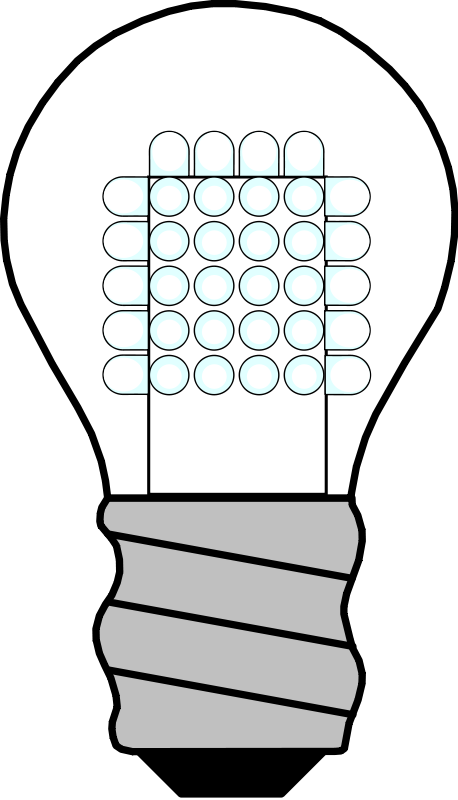
\includegraphics[scale=0.02]{imgs/bulb.png}
 \textbf{Nota} \\
 }%
{\endMakeFramed}

%Work in progress
\newenvironment{workinprogress}{%
  \def\FrameCommand{\colorbox{pink}}%
  \MakeFramed {\FrameRestore}
\lhdbend  \textbf{Work in progress} \\
 }%
{\endMakeFramed}

%Openquestion
\newenvironment{openquestion}{%
  \def\FrameCommand{\colorbox{pink}}%
  \MakeFramed {\FrameRestore}
 \textbf{Domanda aperta} \\
 }%
{\endMakeFramed}

%TODO
\newenvironment{todo}{%
  \def\FrameCommand{\colorbox{pink}}%
  \MakeFramed {\FrameRestore}
 \textbf{TODO} \\
 }%
{\endMakeFramed}

%%%%%%%%%%%%%%%%%%%%%%%%%%%%%%%%
%%%%%%%%%%%% HEADER %%%%%%%%%%%%
%%%%%%%%%%%%%%%%%%%%%%%%%%%%%%%%
\pagestyle{fancy}
% i comandi seguenti impediscono la scrittura in maiuscolo
% dei nomi dei capitoli e dei paragrafi nelle intestazioni
\renewcommand{\chaptermark}[1]{\markboth{#1}{}}
\renewcommand{\sectionmark}[1]{\markright{\thesection\ #1}}
\fancyhf{} % rimuove l'attuale contenuto dell'intestazione
% e del pi\`e di pagina
\fancyhead[LE,RO]{\bfseries\thepage}
\fancyhead[LO]{\bfseries\rightmark}
\fancyhead[RE]{\bfseries\leftmark}
\renewcommand{\headrulewidth}{0.5pt}
\renewcommand{\footrulewidth}{0pt}
\addtolength{\headheight}{0.5pt} % riserva spazio per la linea
\fancypagestyle{plain}{%
\fancyhead{} % ignora, nello stile plain, le intestazioni
\renewcommand{\headrulewidth}{0pt} % e la linea
}


%%%%%%%%%%%%%%%%%%%%%%%%%%%%%%%%
%%%%%%%%%%%% COLORS %%%%%%%%%%%%
%%%%%%%%%%%%%%%%%%%%%%%%%%%%%%%%
\definecolor{code}{gray}{0.3}


%%%%%%%%%%%%%%%%%%%%%%%%%%%%%%%%
%%%%%%%%%%%% NUMBERS %%%%%%%%%%%
%%%%%%%%%%%%%%%%%%%%%%%%%%%%%%%%
\setcounter{tocdepth}{3}
\setcounter{secnumdepth}{3}


%%%%%%%%%%%%%%%%%%%%%%%%%%%%%%%%
%%%%%%%%%%% DOC DATA %%%%%%%%%%%
%%%%%%%%%%%%%%%%%%%%%%%%%%%%%%%%
\title{Appunti di MNO}
\author{Gruppo Informatici Rampanti}
\date{ott 2010 - mag 2011}

\pdfinfo{%
  /Title    (Appunti di MNO)
  /Author   (Andrea Cimino e Lorenzo Muti)
  /Creator  (Andrea Cimino)
  /Producer (Lorenzo Muti)
  /Subject  (MNO)
  /Keywords (MNO)
}


%%%%%%%%%%%%%%%%%%%%%%%%%%%%%%%%
%%%%%%%%%%%%% UTILS %%%%%%%%%%%%
%%%%%%%%%%%%%%%%%%%%%%%%%%%%%%%%
% binary symbols
\newcommand{\modder}{\vdash _{R}}

% vertical gaps
\newcommand{\askip}{\vspace{0.5cm}}
\newcommand{\bskip}{\vspace{1.0cm}}

% various symbols
\newcommand{\qedhere}{\ensuremath{\Box}}
\newcommand{\qed}{\hfill \ensuremath{\Box}}

% substitution
\newcommand{\subst}[2]{^{#1} / _{#2}}

% denotational semantics function names
\newcommand{\bbracket}[1]{\left\llbracket #1 \right\rrbracket}

\newcommand{\aexpr}{\mathcal{A}}
\newcommand{\bexpr}{\mathcal{B}}
\newcommand{\cexpr}{\mathcal{C}}
\newcommand{\Aexpr}[1]{\mathcal{A} \bbracket{#1}}
\newcommand{\Bexpr}[1]{\mathcal{B} \bbracket{#1}}
\newcommand{\Cexpr}[1]{\mathcal{C} \bbracket{#1}}

\newcommand{\semdomset}[1]{(V_{#1})_{\bot}}

% semantic evaluations
\newcommand{\opereval}[3]{\left\langle #1, #2 \right\rangle \rightarrow #3}
\newcommand{\denaeval}[3]{\Aexpr{#1} #2 = #3}
\newcommand{\denbeval}[3]{\Bexpr{#1} #2 = #3}
\newcommand{\denceval}[3]{\Cexpr{#1} #2 = #3}

% rotated sqsubseteqs
\newcommand{\upsqsubseteq}{ $\begin{rotate}{90} $\sqsubseteq$ \end{rotate}$ }
\newcommand{\downsqsubseteq}{ $\begin{rotate}{270} $\sqsubseteq$ \end{rotate}$ }

% Space after paragraph declaration
\makeatletter
\renewcommand\paragraph{\@startsection{paragraph}{4}{\z@}%
  {-3.25ex\@plus -1ex \@minus -.2ex}%
  {1.5ex \@plus .2ex}%
  {\normalfont\normalsize\bfseries}}
\makeatother



% fast theorem and definition
\newcommand{\ftheo}[1]{\colorbox{YellowGreen}{#1}}
\newcommand{\fdefn}[1]{\colorbox{SkyBlue}{#1}}

\theoremstyle{break}
\theoremsymbol{\ensuremath{\clubsuit}}
\theoremseparator{\newline}
\newshadedtheorem{proc}[theo]{Procedura}

% bold math!
\newcommand{\bm}[1]{\mbox{\boldmath{$#1$}}}

\newcommand{\positive}[1]{\textbf{\color{green} +} #1}
\newcommand{\negative}[1]{\textbf{\color{red} -} #1}


\newtheoremlisttype{tab}%
{\begin{tabular*}{\linewidth}{@{}lrl@{\extracolsep{\fill}}r@{}}}%
{##1&##2&##3&##4\\}%
{\end{tabular*}}
\begin{document}
}
\providecommand{\outbpdocument}{\end{document}}
\else
\providecommand{\inbpdocument}{}
\providecommand{\outbpdocument}{}
\fi



\inbpdocument 

% 11 Marzo
\chapter{Il problema lineare dei minimi quadrati}

\section{Metodo delle equazioni normali}

Sia
\begin{equation}
  \label{eq:06minq01} Ax = b
\end{equation} 
un sistema lineare in cui la matrice $A \in \mathbb{C}^{m \times n}$ 
dei coefficienti \`e tale che $m \geq n$.  Se $m > n$, il sistema
(\ref{eq:06minq01}) ha pi\`u equazioni che incognite e si dice
sovradeterminato. Se il sistema (\ref{eq:06minq01}) non ha soluzione,
fissata una norma vettoriale $||\;.\;||$, si ricercano i vettori $x
\in \mathbb{C}^{n}$ che minimizzano la quantit\`a $||Ax − b||$.  In
norma 2, il problema diventa quello di determinare un vettore $x \in
\mathbb{C}^n$ tale che
 \begin{equation}
 \label{eq:06minq02} || Ax − b ||_{2} = \displaystyle \min_{y \in
\mathbb{C}^{n}} || Ay − b||_{2} = \gamma
 \end{equation} Tale problema viene detto problema dei minimi
quadrati.  Il seguente teorema caratterizza l'insieme $X$ dei vettori
$x \in \mathbb{C}^n$ che soddisfano alla (\ref{eq:06minq02}).

\begin{theo} Valgono le seguenti propriet\`a:
   \begin{enumerate}
   \item $x \in X$ se e solo se
     \begin{equation}
         \label{eq:06minq03} A^H Ax = A^Hb
     \end{equation} Il sistema (\ref{eq:06minq03}) viene detto sistema
delle equazioni normali o sistema normale.

\item $X$ \`e un insieme non vuoto, chiuso e convesso.

\item L'insieme $X$ si riduce ad un solo elemento $x^∗$ se e solo se
la matrice $A$ ha rango massimo.
\item Esiste $x^∗ \in X$ tale che
  \begin{equation}
\label{eq:06minq04} || x^{*}||_{2} = \displaystyle \min_{x \in X}
||x||_{2}
  \end{equation} Il vettore $x^{*}$ \`e l'unico vettore di $X$ che
appartiene a $N(A^{H}A)^{\bot}$ ed \`e detto \emph{soluzione di minima
norma}
   \end{enumerate}
\end{theo}

\begin{thproof}
  \begin{enumerate}
  \item Siano
$$ S(A) = \{ y \in \mathbb{C}^{m}: y = Ax 
\text{ per qualche } x \in \mathbb{C}^{m} \}$$ e
$$
S(A)^{\bot} = \{ z \in \mathbb{C}^{m} \; : \; z^{H}y = 0, \forall y
\in S(A) \}
$$
il sottospazio di $\mathbb{C}^m$ immagine di $A$, e il sottospazio
ortogonale a $S(A)$ (si vedano i paragrafi 2 e 6 del capitolo 1).  Il
%dio cane mettete i \ref!!!
vettore $b$ pu\`o essere cos\`i decomposto
 $$ b = b_1 + b_2, \quad \text{dove } 
 b_1 \in S(A) \text{ e } b_2 \in S(A)^{\bot} $$

per cui il residuo
$$ r=b_1 - Ax + b_2 = y + b_2, \quad
\text{dove } y=b_1 - Ax \in S(A) \text{ e } b_2 \in S(A)^{\bot}$$

vale
$$ ||r||_{2}^{2} = (y + b_2)^{H} (y + b_2) = 
||y||_{2}^{2} + ||b_2||_{2}^{2}$$ 

in quanto $y^{H}b_2 = b_2^{H}y=0$. Per minimizzare $||r||_{2}^{2}$,
non possiamo agire su $b_2$ poich\'e \`e costante, mentre possiamo
porre a zero $y$ che dipende da $x$, il che equivale a porre $b_1 = Ax$, 
che \`e verificato per qualche $x$ dato che $b_1$ appartiene al
sottospazio immagine di $A$. \\
A questo punto otteniamo 
$$ ||r||_{2}^{2} = ||b_2||_{2}^{2}$$

vero se e solo se il vettore $r$ appartiene a $S(A)^{\bot}$ ed \`e quindi ortogonale
alle colonne di $A$, cio\'e
$$A^{H}r = A^{H} (b − Ax) = 0$$
Ne segue quindi che $x \in X$ se e solo se $x$ \`e soluzione di
(\ref{eq:06minq03}).  Inoltre risulta $\gamma^{2} = ||b_2||_{2}^{2}$

Nel caso di $\mathbb{R}^2$ con una matrice $A$ di rango $1$ si pu\`o
dare la seguente interpretazione geometrica, illustrata nella figura
7.1. Il vettore $b = r − Ax$ risulta decomposto in un sol modo nel
vettore $b_2 = r \in S(A)^{\bot}$ e nel vettore $b_1 = Ax \in S(A)$.
Il vettore $Ax$ \`e quindi la proiezione ortogonale del vettore $b$
sul sottospazio generato dalle colonne di $A$.
\begin{todo} Inserire immaginina
\end{todo}

\item L'insieme $X$ non \`e vuoto dato che, per quanto detto
precedentemente, $Ax=b_1$ ha soluzione per come abbiamo scelto $b_1$.\\
% VERSIONE DELLE DISPENSE
% Se $x_0$ \`e tale che
% $$A^{H}Ax_0 = A^{H}b $$
% allora risulta
% $$ X = \{ x \in \mathbb{C}^{n} \; : \; x = x_0 + v, v
%  \in N(A^{H}A) \}$$ Quindi $X$ \`e una variet\`a lineare affine,
% parallela ad $N(A^{H} A)$, passante per $x_0$ , e poich\'e $N(A^{H}
% A)$ \`e chiuso e convesso, $X$ un insieme chiuso e convesso.\\

% VERSIONE FATTA A LEZIONE
Mostriamo ora che $X$ è chiuso e convesso:
\begin{enumerate}
\item caso $rank(A) = n$ \\ 
  $A^{H}A$ è definita positiva non singolare, $A^{H}Ax = A^{H}b$ ha
  soluzione unica ed $X$ è formato da un solo vettore.
\item caso $rank(A) < n$\\ 
  $A^{H}A$ è semi-definita positiva, $det(A^H A) = 0$,
  abbiamo infinite soluzioni delle forma
  $$X = \{ x = x_0 + v\} \qquad v \in Ker(A^{H}A)$$
  e poich\'e $N(A^{H} A)$ \`e chiuso e convesso, $X$ un insieme chiuso
  e convesso.\\

  Ad esempio poniamo che il rango sia 1 in $\mathbb{R}^2$ con $n =2$,
  allora $dim(Ker(A^{H}A)) = 1$ e $rank(A^{H}A) = 1$, l'insieme delle
  soluzioni $X$ è una retta, che è un insieme chiuso e convesso.
\end{enumerate}

\item per quanto detto al secondo punto se $A$ ha rango massimo, $X$
  contiene un solo elemento. In tal caso l'insieme $N (A^{H} A)$ \`e 
  costituito dal solo elemento nullo.

\item l'esistenza della soluzione di minima norma \`e ovvia
  nel caso in cui $X$ si riduce al solo elemento $x$.\\
  Invece se $A$ non ha rango massimo, per quanto detto al secondo punto, $X$
  è formato da infiniti elementi ed esiste $x^{*} \in X$ tale che
  $||x^{*}|| = \min_{X} ||x||$ e $x^{*}$ è l'\emph{unica} soluzione
  appartenente a $Ker(A^H A)^{\bot}$.\\

  Versione più approfondita dalle dispense:\\
  Se $X$ non si riduce al solo elemento $x^{∗}$ , sia $x_0 \in X$ e si consideri
  l’insieme
  $$ B = \{ x \in \mathbb{C}^{n}\; : \; ||x||_{2} \leq ||x_0||_2 \}$$
  Poich\'e, se $x \in X$, ma $x \notin B$, risulta $||x||_{2} >
  ||x_0||_{2}$, allora
  $$  \displaystyle 
  \min_{x \in X} ||x||_{2} = \min_{x \in X \cap B} ||x||_{2}
  $$
  L'insieme $X \cap B$ \`e un insieme non vuoto, limitato e chiuso, in
  quanto intersezione di insiemi chiusi, e quindi compatto; essendo la
  norma una funzione continua, esiste un $x^∗ \in X \cap B$ per cui vale
  la (\ref{eq:06minq04}).

  Inoltre $x^*$ \`e l'unico vettore di $X$ appartenente a a
  $N(A^{H}A)^{\bot}$ Infatti esistono e sono unici $ y \in N (A^{H} A)$
  e $z \in N (A^{H} A)^{\bot}$ tali che $x^{∗} = y + z$ Poich\'e $x^*$
  \`e soluzione di (\ref{eq:06minq03}).  $ A^{H} A(y + z) = A^H b$, da
  cui $A^H Az = A^H b$ e quindi z \`e soluzione del problema
  (\ref{eq:06minq02}).  Se $y$ non fosse uguale a 0, $z$ avrebbe norma 2
  minore di $||x^*||$ , ci\`o \`e assurdo perch\'e $x^∗$ \`e la
  soluzione di minima norma: ne segue che $x^* = z \in N (A^H A)^{\bot}$.

  Nel caso di $\mathbb{R}^2$ con una matrice $A$ di rango 1, si pu\'o
  dare l’interpretazione geometrica illustrata nella figura in cui \`e
  riportata la variet\`a $X$, parallela alla variet\`a $N (A^H A)$.  Il
  punto $x_0$ un qualunque punto di $X$. Il punto $x^∗$ \`e quello di
  minima norma e quindi quello pi\`u vicino all’origine $O$ dello spazio
  $\mathbb{C}$
\end{enumerate}
\end{thproof}

\paragraph{Risoluzione tramite Cholesky} 
Se la matrice A ha rango massimo, allora la soluzione del problema dei
minimi quadrati pu\`o essere ottenuta risolvendo il sistema
$$A^{H}Ax = A^{H}b$$
In tal caso, poich\'e la matrice $A^{H}{A}$ \`e definita positiva
(\ref{prop:def-pos}), si pu\`o utilizzare per la risoluzione il metodo
di Cholesky \ref{sec:fatt-cholesky}.
Determinata la matrice triangolare inferiore tale che
$$LL^{H} =A^{H} A$$
la soluzione $x^{*}$ di $A^{H}Ax = A^{H}b$ viene calcolata risolvendo
successivamente i due sistemi di ordine $n$ con matrice di
coefficienti triangolare
$$Ly = A^H b$$
$$L^H x = y$$

Se la matrice $A$ non ha rango massimo, non si pu\`o risolvere il 
sistema 
(\ref{eq:06minq03}) con il metodo di Cholesky, ma si pu\`o
 applicare il metodo di Gauss con la variante del massimo pivot.

\paragraph{Costo}
Nel caso di una soluzione:
\begin{itemize}
\item Calcolo di $A^{H}A$ :$ n^{2}m/2$ per la costruzione della
matrice hermitiana
\item Cholesky: $n^{3}/6$ per la risoluzione del sistema
\end{itemize} In totale quindi il costo \`e: $n^{2}((m/2) + (n/6))$

\begin{workinprogress} 
Condizionamento, definito solo per le quadrate,
per le rettangolari si passa per SVD,
$$ \mu(A) = ||A|| ||A^{-1}||$$
$$  \mu(A^{H}A) = \mu^{2}(A)$$
Cholesky è stabile
\end{workinprogress}

\section{Metodo QR} 
Si esamina ora un altro procedimento, detto metodo QR, che opera
direttamente sulla matrice A fattorizzandola nella forma QR
\ref{fatt:QR}, dove $Q$ \`e una matrice ortogonale.  In particolare,
poich\'e si sta lavorando nel campo complesso, $Q$ \`e unitaria. \\
Si supponga dapprima che la matrice $A \in C^{m\times n} $ abbia rango
massimo, $k = n \leq m$.  Si applica il metodo di Householder alla
matrice $A$, ottenendo una successione di matrici di Householder 
\ref{sec:householder}.
$$ P^{(k)} \in \mathbb{C}^{m \times m }, k =1, \ldots, n$$
Posto $Q^{H} = P^{(1)} P^{(2)}\ldots P^{(n)}$ risulta
\begin{equation}
  \label{eq:06minq05} A=QR
\end{equation} 
dove la matrice $R \in \mathbb{C}^{m \times n}$ ha la forma

\begin{equation}
  \label{eq:06minq06} R = \left[
\begin{array}{l} R_1 \\ \\ 0
\end{array} \right]
\begin{array}{l} \}n \text{ righe} \\ \\ \}m-n \text{ righe}
\end{array}
\end{equation}

ed $R_1$ \`e una matrice triangolare superiore non singolare in quanto
$A$ ha rango massimo. Dalla (\ref{eq:06minq05}) si ha

\begin{equation}
  \label{eq:06minq07} 
  || Ax - b ||_2 = ||QRx - b||_2 \underbracket{=}_{*)} 
  ||QRx - QQ^{H}b||_2 = ||Q(Rx - Q^{H}b)||_2 = ||Rx - Q^{H}b||_2 = 
  ||Rx - c||_2
\end{equation}
*) Le matrici unitarie preservano la norma 2 (\ref{prop:unitarie})\\

dove $c = Q^H b$. Partizionando il vettore $c$ nel modo seguente
$$
  c = \left[
\begin{array}{l} c_1 \\ \\ c_2
\end{array} \right]
\begin{array}{l} \}n \text{ componenti} \\ \\ \}m-n \text{ componenti}
\end{array}
$$
per la (\ref{eq:06minq06}) vale
$$
Rx - c = \left[
\begin{array}{c} R_1 x -c_1 \\ -c_2
\end{array} \right]
$$
per la (\ref{eq:06minq07}) risulta
$$\min_{x \in \mathbb{C}^{n}}||Ax-b ||_{2}^{2}
= \min_{x \in \mathbb{C}^{n}}||Rx-c ||_{2}^{2} = \min_{x \in
\mathbb{C}^{n}}[||R_1x-c_1 ||_{2}^{2} + ||c_2||_2^2] = ||c_2||_2^2 +
\min_{x \in \mathbb{C}^{n}} ||R_1x - c_1 ||_{2}^{2}
 $$
Poich\'e $R_1$ \`e non singolare, la soluzione $x^{*}$ del sistema
lineare
\begin{equation}
 \label{eq:06minq08} R_1x = c_1
\end{equation} \`e tale che
$$
\min_{x \in \mathbb{C}^{n}} ||R_1 x - c_1||_2 = ||R_1 x^{*} -c_1||_2 =
0
$$
ne segue che $x^*$ \`e la soluzione del problema
$$|| Ax − b ||_{2} = \displaystyle \min_{y \in
\mathbb{C}^{n}} || Ay − b||_{2} = \gamma$$ e si ottiene
$$\gamma = ||c_2||_2$$

\begin{notes} Mi sembra che la parte parte sull'evitare il calcolo
delle matrici $P^{(k)}$ e $Q$ non l'ha spiegata, ma la scrivo per
completezza.
\end{notes} Analogamente al caso della risoluzione dei sistemi
lineari, il metodo pu\`o essere applicato senza calcolare
effettivamente n\'e le matrici $P^{(k)}, k =1\ldots n$, n\'e la
matrice $Q$.  Si pu\`o procedere infatti nel modo seguente: sia
$$P^{(k)} = I - \beta_{k} v_k v_k^{H}, \quad
k=1, \ldots n$$ Consideriamo la matrice
$$T^{(1)} = [A \; | \; b]$$
e si costruisce le successioni delle matrici $T^{(k)}$ tali che
$$
T^{(k+1)} = P^{(k)}T^{(k)} = T^{(k)} - \beta_k v_k v_k^{H} T^{(k)}
$$
Al termine dopo $n$ passi si ottiene la matrice
$$ T^{(n+1)} = [R \; | \; c ] $$

\subsection{Casi e Costi} \subparagraph{Rango massimo} Nel caso
$det(R_1) \neq 0 \; \Longleftrightarrow \; rank(A) =n$, abbiamo
un'unica soluzione. La complessit\`a computazionale \`e data da:
\begin{itemize}
 \item Calcolo $QR$: $n^{2}(m-n/3) \approx n^{2}m$ (circa il doppio di
Cholesky)
\item Risolvere $x = R_1^{-1} C_1$: $n^2$ operazioni
\end{itemize} In generale quindi $QR$ richiede pi\`u operazioni, ma se
$m=n$ i due metodi hanno lo stesso costo.

\subparagraph{Rango $<n$: metodo del massimo pivot} 
In questo caso esistono infinite soluzioni, ed \`e necessario
provvedere ad una riformulazione del problema nel seguente modo
$$ A\Pi = QR$$ 
dove $\Pi$ \`e una matrice di permutazione delle colonne.  Infatti se
la matrice $A$ non ha rango massimo, la matrice $R_1$ ottenuta ha
almeno un elemento diagonale nullo e quindi non \`e possibile
calcolare la soluzione del sistema (\ref{{eq:06minq08}}). \\
Questa difficolt\`a viene superata applicando il metodo QR con la
tecnica \emph{del massimo pivot} (\ref{qr-max-pivot})per colonne nel
modo seguente: al $k$-esimo passo, costruita la matrice $A^{(k)}$
della forma
$$
A^{(k)} = \left[
  \begin{array}{lll} 
    C^{(k)} &  & D^{(k)}                                  \\ 
            &  &                                          \\ 0 &  & B^{(k)}
  \end{array} 
\right]
\begin{array}{l} 
  \} k-1 \text{ righe}                                    \\ 
                                                          \\ 
  \}m-k+1 \text{ righe}
\end{array}
$$

si determina la colonna di $B^{(k)}$ la cui norma 2 \`e massima. Sia
$j, 1 \leq j \leq n-k+1$ l'indice di tale colonna. Se $j = 1$, si
scambiano fra loro la $k$-esima e la $(k + j − 1)$-esima colonna della
matrice $A^{(k)}$ . Quindi si applica la matrice elementare $P^{(k)}$
alla matrice con le colonne cos\`i permutate.  Se il rango di A \`e $r
< m$, questo procedimento termina dopo $r$ passi, e si ottiene una
decomposizione del tipo
$$ A\Pi = QR$$ 
dove $\Pi \in \mathbb{R}^{n \times n}$ \`e una matrice di
permutazione, $Q \in \mathbb{C}^{m \times m}$ \`e una matrice unitaria
ed $R$ \`e della forma
$$
 A^{(k)} = \left[
\begin{array}{lll} R_1 & & S \\ & & \\ O & & O
\end{array} \right]
\begin{array}{l} \} r \text{ righe} \\ \\ \}m-r \text{ righe}
\end{array}
$$
in cui $R_1 \in C^{r \times r}$ \`e triangolare superiore non
singolare e $S \in \mathbb{C}^{r \times (n -r)}$. Gli elementi
diagonali di $R_1$ risultano positivi ed ordinati in ordine modulo non
crescente .
\begin{notes} Il professore su questo ultimo punto \`e stato vago, ma
sul libro \`e spiegato tutto per bene.
\end{notes}

\begin{workinprogress} \textbf{Cosa avra mai voluto dire?} \\ Costo:
$(m-k) (n-k) + (m-k)(n-k)$ \\ Sommando su tutti i $k$
$$
\displaystyle 2 \sum_{k=1}^{n} (m-k)(n-k)
$$
$$i =n-k \quad i =1, \ldots, n \quad k = n-i$$
$$ 
2 \displaystyle \sum_{i=1}^{n} (m-n+i)i = 2 (\displaystyle
\sum_{i=1}^{n} (m-n) i + \displaystyle i^{2}) = 2 (( m-n)
\frac{n^{2}}{2} + \frac{n^3}{3}) = (m-n)n^{2} + \frac{2}{3}n^{3}
$$   
\end{workinprogress}

\section{Norme di matrici non quadrate} Per comprendere i successivi
metodi, \`e necessario introdurre questo concetto.  Sia $A \in
\mathbb{C}^{m\times n}$. Le norme matriciali indotte, come gi\`a visto
in precedenza, vengono definite per mezzo della relazione
$$ || A|| = \max_{||x||' = 1} ||Ax ||'' = \sup_{x \neq 0}
\frac{||Ax||}{||x||}
$$
dove $|| \; . \; ||$ e $|| \; . \; ||''$ sono norme vettoriali
rispettivamente su $\mathbb{C}^{n}$ e $\mathbb{C}^{m}$. \\ Estendiamo
questo concetto sulla matrici $m \times n$, usando la norma 2,
usandola in $|| \; . \; ||$ e $|| \; . \; ||''$.  Si dimostra che:
$$ || A||_{2} = \sqrt{\rho(A^{H}A)}
\qquad \text{($\rho$: raggio spettrale)}
$$
Utilizzando invece la norma, di Frobenius otteniamo
$$ ||A||_{F} = \sqrt{tr(A^{H}A)} =
\sqrt{\displaystyle \sum_{i,j}|a_{ij}|^{2} } \qquad \text{(tr =
traccia)}
$$ 
Questa non è una norma indotta.

\paragraph{Invarianza della norme} Se $U \in \mathbb{C}^{m \times m}$
e $V \in \mathbb{C}^{n\times n}$ sono matrici unitarie, poiché
$$ (U^{H}AV)^{H}(U^{H}AV) = V^{H}A^{H}AV$$
risulta
$$|| U^{H}AV||_{2} = \sqrt{\rho(A^{H}A)} = ||A||_{2}$$
La stessa cosa vale per la norma di Frobenius. \\ \\ A lezione
Bevilacqua ha scritto:
$$ || AU||_{2}^{2} = \rho (U^{H} A^{H}A U)
= \rho(A^{H}A) = ||A||_{2}^{2}
$$
$$ ||UA ||_{2}^{2} = \rho(A^{H} U^{H}UA)
= \rho(A^{H}A) = ||A||_{2}^{2}$$

\section{SVD: Decomposizione ai valori singolari di una matrice }
Vedremo un metodo per risolvere il problema dei minimi quadrati,
tramite un nuovo tipo di fattorizzazione: la SVD.  Il pregio di questo
metodo \`e che vengono coinvolte matrici unitarie che hanno garanzie di
stabilità. \\ 
Assomiglia ad una trasformazione per similitudine ma non lo \`e.

% TODO
% Ricordiamo che se $A$ \`e hermitiana e semidefinita positiva, allora
% ci siamo riportati al metodo
% $$ A = QDQ^{H} \qquad D = diag(\lambda_i)$$
% $\lambda_i$ autovalori, colonne di Q sono gli autovettori. \\

\begin{theo} Sia $A \in \mathbb{C}^{m \times n}$. Allora esistono una matrice
unitaria $U \in \mathbb{C}^{m \times m}$ ed una matrice unitaria $V
\in \mathbb{C}^{n \times n}$ tali che
\begin{equation}
  \label{eq:06minq09} A = U \Sigma V^{H}
\end{equation} dove la matrice $\Sigma \in \mathbb{R}^{m \times n}$ ha
elementi $\sigma_{ij}$ nulli per $i \neq j$ e per $i =j$ ha elementi
$\sigma_{ii} = \sigma_i$ con
$$
\sigma_1 \geq \sigma_2 \geq \ldots \sigma_p \geq 0, \quad p =
\min\{m,n\}
$$
La decomposizione \`e detta decomposizione ai valori singolari della
matrice $A$, mentre i valori $\sigma_i$, per $i = 1, \ldots , p,$ sono
detti \textbf{valori singolari} di $A$. Indicate con $u_i , i = 1,
\ldots , m,$ e $v_i , i = 1, \ldots , n$, le colonne rispettivamente
di $ U$ e di$ V$ , i vettori $u_i$ e $v_i$ , $i = 1, \ldots , p,$ sono
detti rispettivamente \textbf{vettori singolari sinistri} e
\textbf{vettori singolari destri} di $A$.  La matrice $\Sigma$ \`e
univocamente determinata, anche se le matrici $U$ e $V$ non lo sono.
\end{theo}

\begin{figure}[hb] \centering
$$
\Sigma =
\begin{pmatrix} 
  \sigma_1 & 0        & 0      & 0      & 0        \\ 
  0        & \sigma_2 & 0      & 0      & 0        \\
  0        & 0        & \ddots & 0      & 0        \\ 
  0        & 0        & 0      & \ddots & 0        \\ 
  0        & 0        & 0      & 0      & \sigma_n \\
\end{pmatrix} $$

$$ \sigma_i \in \mathbb{C}
\quad \sigma_1 \geq \sigma_2 \geq \ldots \geq \sigma_n \geq 0$$
\caption[Struttura della matrice $\Sigma$]{Struttura della matrice
  $\Sigma$}
\end{figure}

\begin{thproof} Si considera per semplicit\`a il caso $m \geq n$ (se
$m < n$, si sostituisce $A$ con $A^H$). Si procede dimostrando per
induzione su $n$ che la tesi vale per ogni $m \geq n$.  Per $n = 1$
\`e $A = a \in \mathbb{C}^m$.  Si pone $\sigma_1 = ||a||_2$ e si
considera come matrice $U$ la matrice di Householder tale che $Ua =
\sigma_1e_1$. La matrice $V$ \`e la matrice $V = [1]$.  \\ Per n > 1
si dimostra che se la tesi vale per le matrici di $C^{k \times
(n-1)}$, con $k \geq n-1$¸ allora vale per le matrici di $C^{k \times
(n)}$ con $m \geq n$ . Sia $ x \in \mathbb{C}^{n}$ tale che $||x||_2 =
1 $ e $||A||_2 = ||Ax||_2$.  Si consideri il vettore
 $$y = \dfrac{Ax}{||Ax||_2} \in \mathbb{C}^{n}$$

Allora $||y||_2 = 1$ e $Ax = \sigma_1y,$ con $\sigma_1 =
||A||_2$. Siano poi $V_1 \in \mathbb{C}^{n \times n} $ e $U_1 \in C^{m
\times m}$ matrici unitarie le cui prime colonne sono uguali
rispettivamente a $x$ e $y$. Poich\'e
$$U_1^{H} AV_1e_1 = U_1^H Ax 
= U_1^{H} \sigma_1 y = \sigma_1[1; 0; \ldots ; 0]^T $$ \`e
\begin{notes}
Quest'ultimo passaggio si spiega col fatto
che $U_1$ \`e unitaria, allora anche la sua trasposta
coniugata \`e unitaria, allora $U^{h} U = I$, Se al posto
di $U$ prendiamo proprio $y$, ottieniamo la prima colonna
della matrice identit\`a
\end{notes}

$$
 A_1 = U_1^{H}AV_1 = \left[
\begin{array}{lll} \sigma_1 & & w^{H} \\ & & \\ 0 & & B
\end{array} \right]
\begin{array}{l} \}1 \text{ riga} \\ \\ \}m-1 \text{ righe}
\end{array}
$$
in cui $w \in \mathbb{C}^{n−1}, B \in \mathbb{C}^{(m−1)\times(n−1) }$
e $\mathbf{0} \in \mathbb{C}^{m−1}$.  Si dimostra ora che $w = 0$. Si
supponga per assurdo ch e $w \neq 0$ e si consideri il vettore $z =
\left[
 \begin{array}{l} \sigma_1 \\ w
\end{array} \right] \neq \mathbf{0} $ per cui
$$
A_1z = \left[
  \begin{array}{c} \sigma_1^{2} + w^{H}w \\ Bw
  \end{array} \right]
$$
 Si ha

$$
||A_1 z||_2^2 = ||z||_2^4 + || Bw||_2^{2} \geq ||z||_2^4
$$
da cui, dividendo per $||z||_2^2$ si ottiene
$$
\dfrac{||A_1z||_2^2}{||z||_2^2} \geq ||z||_2^2
$$
e quindi
\begin{equation}
  \label{eq:06minq10} ||A_1||_2^{2} \geq \sigma_1^{2} + w^{H}w.
\end{equation}
D'altra parte \`e $||A_1||_2 = ||A||_2$ 
 in quanto $A_1$ \`e ottenuta da $A$ con trasformazioni unitarie e
quindi
 \begin{equation}
   \label{eq:06minq11} ||A_2||_2 =\sigma_1.
 \end{equation} Dal confronto fra la (\ref{eq:06minq10}) e la
(\ref{eq:06minq11}) segue l’assurdo. Quindi

$$
A_1 \left[
\begin{array}{ccc} \sigma_1 & & \mathbf{0}^{H}\\ & & \\ \mathbf{0} & &
B \\
\end{array} \right]
$$
Dalla (\ref{eq:06minq11}) segue che
\begin{equation}
  \label{eq:06minq12} \sigma_1 \geq ||B||_2
\end{equation} Infatti
$$
\sigma_1^{2} = ||A_1||_2^{2} =  \rho(A_1^{H}A_1) = \rho \left( \left[
\begin{array}{ccc} \sigma_1^2 & & \mathbf{0}^{H}\\ & & \\ \mathbf{0} &
& B^{H}B
\end{array} \right] \right) = \max [\sigma_1^{2}, \rho(B^{H}B)] \geq
\rho (B^H B) = ||B||_2^2 .
$$
Poich\'e $B \in C^{(m−1)\times(n−1)} $e $m − 1 \geq n − 1$, per
l'ipotesi induttiva si ha
$$
U_2^{H}BV_2 = \Sigma_2
$$
dove le matrici $U_2 \in \mathbb{C}^{(m−1)\times(m−1)}$ e $V_2 \in
\mathbb{C}^{(n−1)\times(n−1)}$ sono unitarie e $\Sigma_2 \in
\mathbb{R}^{(m−1)\times(n−1)}$ ha elementi $\sigma_2 \geq \ldots \geq
\sigma_p$ . Poich\'e $\sigma_2 = ||B_2|| \leq \sigma_1$ per la
(\ref{eq:06minq12}), la tesi segue con
$$
U= U_1 \left[
\begin{array}{ccc} 1 & & \mathbf{0}^{H}\\ & & \\ \mathbf{0} & & U_2
\end{array} \right], \; V = V_1 \left[
\begin{array}{ccc} 1 & & \mathbf{0}^{H}\\ & & \\ \mathbf{0} & & V_2
\end{array} \right], \; \Sigma = \left[
\begin{array}{ccc} \sigma_1 & & \mathbf{0}^{H}\\ & & \\ \mathbf{0} & &
\Sigma_2
\end{array} \right]
$$

Le matrici $U$ e $V$ non sono univocamente determinate: infatti se
$$ A = U \Sigma V^{H}$$
\`e una decomposizione ai valori singolari di $A$, e se $S \in
\mathbb{C}^{n \times n}$ una matrice di fase e $Z \in
\mathbb{C}^{(m-n) \times (m-n)}$ \`e una matrice unitaria, anche

$$
A = U \left[
\begin{array}{ccc} S & & 0\\ & & \\ 0 & & Z
\end{array} \right] \Sigma S^{H}V^{H}
$$
\`e una decomposizione ai valori singolari di $A$.  Inoltre se
$\sigma_i = \sigma_{i+1} = \ldots = \ \sigma_{i+j}$ , per $j \geq 1$,
detta $P$ una qualunque matrice unitaria di ordine $j + 1$ e
considerata la matrice diagonale a blocchi
$$
Q= \left[
\begin{array}{ccc} I_{i-1} & O & O \\ & & \\ O & P & O \\ & & \\ O & O
& I_{n-j-i} \\
\end{array} \right]
$$
si ha che

$$
A= U \left[
\begin{array}{cc} Q & O \\ & \\ O & I_{m-n}
\end{array} \right] \Sigma Q^{H}V^{H}
$$
\`e una decomposizione ai valori singolari di $A$
\end{thproof} Dal teorema segue che
\begin{equation}
  \label{eq:06minq13} A = U\Sigma V^{H} = \displaystyle \sum_{i=1}^{p}
\sigma_i u_i v_i^{H}
\end{equation}

$$
\left.
\begin{array}{c} Av_i = \sigma_i u_i \\ A^{H} u_i = \sigma_i v_i
\end{array} \right\}, i=1,\ldots, p
$$
\begin{workinprogress}
\paragraph{Costi}
\begin{itemize}
 \item  Diagonalizzazione: $A^{H}A$ : $\frac{1}{2}mn^{2}$
 \item $A^{H}A$: $O(n^{3})$
 \item  Fattorizzazione $QR$, costo : $mn^{2}$
\end{itemize}
Normalmente costa $\frac{1}{2} mn^{2}$, usando Golum costa $2mn^{2}$
ma \`e più stabile. (Ricontrollare tutto)  
\end{workinprogress}

\begin{theo}
 % 7.10
\label{eq:06minq33}
 Sia $A \in \mathbb{C}^{m \times n}$ e sia
$$A = U\Sigma V^{H}$$
la sua decomposizione ai valori singolari, dove
$$\sigma_1 \geq \sigma_2 \geq . . .
 \geq \sigma_k > \sigma_{k+1} = \ldots = \sigma_p = 0.
$$
Allora valgono le seguenti propriet\`a
\begin{enumerate}
\item
$$ A = U_k \Sigma_k V_k^{H}
= \displaystyle \sum_{i=1}^{k} \sigma_i u_i v_i^{H} , \quad \text{
dove}
$$
$U_k \in \mathbb{C}^{m\times k}$ \`e la matrice le cui colonne sono
$u_1 , \ldots , u_k$ , \\ $V_k \in \mathbb{C}^{n×k}$ \`e la matrice le
cui colonne sono $v_1 , \ldots, v_k$ , \\ $\Sigma_k \in
\mathbb{R}^{k\times k}$ \`e la matrice diagonale i cui elementi
principali sono
$$ \sigma_1, \ldots \sigma_k$$

\item Il nucleo di $A$ \`e generato dai vettori $v_{k+1} ,\ldots ,
v_n$ .

\item L'immagine di $A$ \`e generata dai vettori $u_1, \ldots , u_k$,
e quindi
$$rank(A) = k$$
\item

 $\sigma_i^{2} , i = 1, \ldots, p$ sono gli autovalori della matrice
$A^H A$ (se $m < n$ i restanti autovalori sono nulli) e quindi
$$
||A||_{F}^{2} = \displaystyle \sum_{i=1}^{k} \sigma_i^{2}
$$
$$||A||_2 = \sigma_1 $$

\item Se $m = n$ e $A$ \`e normale, allora $\sigma_ii = |\lambda_i |,
i = 1, \ldots , n$, dove i $\lambda_i$ sono gli autovalori di $A$, e i
vettori singolari destri e sinistri coincidono con gli autovettori di
$A$.
\end{enumerate}

\end{theo}

\begin{thproof} 
Si supponga per semplicit\`a che $p = n \leq m$ (se $n
> m$ si sostituisce $A$ a con $A^{H}$ ).
\begin{enumerate}
\item La matrice $\Sigma$ ha la forma
$$
\left[
\begin{array}{lll} \Sigma_{k} & & O \\ & & \\ O & & O
\end{array} \right]
\begin{array}{l} \} k \text{ righe} \\ \\ \}m-k \text{ righe}
\end{array}
$$
per cui, partizionando le matrici $U$ e $V$ nel modo seguente
$$U = [U_k | U'_{m−k} ] \qquad V = [V_k | V_{n−k} ]$$
Dalla (\ref{eq:06minq13}) risulta che
\begin{equation}
  \label{eq:06minq14} A = U_k \Sigma_k V_k^{H}
\end{equation}

\item Se $x \in \mathbb{C}^n$ , la condizione $Ax = 0$ per la
(\ref{eq:06minq13}) equivalente alla condizione
$$U \Sigma V^{H} x = 0$$
e, poich\'e U non singolare, ` equivalente a
\begin{equation}
  \label{eq:06minq15} \Sigma V^H x = 0
\end{equation} Il vettore $z = \Sigma V^H x$ pu\`o essere partizionato
nel modo seguente

\begin{equation}
  \label{eq:06minq16} \left[
\begin{array}{l} \Sigma_{k}V_k^{H}x \\ \\ O
\end{array} \right]
\begin{array}{l} \} k \text{ compomenti} \\ \\ \}m-k \text{
componenti}
\end{array}
\end{equation}

per cui la (\ref{eq:06minq15}) pu\`o essere scritta come $\Sigma_k
V_k^{H} x = 0$, ossia $V_k^{H} x = 0$.  Quindi $Ax = 0$ se e solo se
$x$ \`e ortogonale alle prime $k$ colonne di $V$ ed essendo $V$
unitaria, se e solo se $x$ \`e generato dalle restanti colonne e di V
.

\item Dalla (\ref{eq:06minq14}) risulta che
\begin{equation}
  \label{eq:06minq17} y=Ax = U_k \Sigma_k V_k^{H}x = U_kz
\end{equation} dove $z = \Sigma_k V_k^{H}x \in \mathbb{C}^{k}$. Quindi
$y$ \`e generato dalle colonne di $U_k$. Viceversa (20) si ha che,
poich\'e la matrice $\Sigma_kV_k$ \`e di rango massimo, per ogni $x
\in \mathbb{C}^{n} , x \neq 0, $ esiste uno $z \neq 0$ per cui vale la
(21).

\item Dalla (\ref{eq:06minq13}) si ha che
$$A^H A = V\Sigma^H \Sigma V^H$$
dove $\Sigma^{H}\Sigma \in \mathbb{R}^{n\times n}$ \`e la matrice
diagonale i cui elementi principali sono 
$\sigma_1^{2},\ldots, \sigma_p^{2}$. Poich\'e la traccia e il raggio
spettrale di due matrici simili sono uguali, si ha
$$
||A||_F^{2} = tr(A^{H}A) = \displaystyle \sum_{i=1}^{p} \sigma_i^{2} =
\sum_{i=1}^{k} \sigma_i^{2}
$$
e
$$
||A||_{2}^{2} = \rho(A^{H}A) = \sigma_1^{2}
$$
e poich\'e $\sigma_1 > 0$ risulta $||A||_2 = \sigma_1$

\item Se $A$ \`e normale, dalla forma normale di Schur di $A$

$$A = U DU^{H}$$ ,
segue che
$$A^H A = UD^{H} DU^H$$
perci\`o gli autovalori $\sigma_i$ di $A^H A$ sono tali che

$$\sigma_i^{2} = \overline{\lambda}_i \lambda_i = |\lambda_i |^2
\quad \text{ per } i = 1, \ldots,n
$$

\end{enumerate}
 
\end{thproof}

\subsection{Calcolo dei valori e vettori singolari}

Dal teorema (\ref{eq:06minq10}) 
si pu\`o ricavare anche un procedimento per calcolare
i valori e i vettori singolari di $A$. Per semplicit\`a si suppone
 $m \geq  n$ (se fosse  $m < n$ basta riferirsi alla matrice
 $A^H$ ). Questo procedimento si articola nei seguenti passi:
 \begin{enumerate}
 \item   si calcolano gli autovalori e gli autovettori,
 normalizzati in norma 2, della matrice $A^H A$ e si considera la
 seguente decomposizione in forma normale di Schur della matrice
$ A^H A$
\begin{equation}
  \label{eq:06minq18}
A^H A = QDQ^H , D \in \mathbb{R}^{n\times n} , Q \in 
\mathbb{C}^{n \times n}   
\end{equation}
in cui gli elementi principali di $D$ sono gli autovalori in 
ordine non crescente di $A^H A$ e $Q$ \`e la corrispondente 
matrice degli autovettori ($Q$ \`e unitaria) (un
metodo stabile per calcolare la decomposizione 
(\ref{eq:06minq18}) sar\`a
 descritto nel  paragrafo 9);

\item
 si calcola la matrice
 \begin{equation}
   \label{eq:06minq19}
  C = AQ \in \mathbb{C}^{m \times n} 
 \end{equation}
e si determina, utilizzando la tecnica del massimo pivot 
per colonne, la fattorizzazione $QR$ della matrice
\begin{equation}
  \label{eq:06minq20}
  C\Pi  = UR = U 
\left[
\begin{array}{c}
R_1  \\
     \\
O
\end{array}
\right]
\end{equation}
dove $\Pi \in \mathbb{R}^{n \times n}$ \`e una matrice di
permutazione, $U \in C^{m \times m}$ \`e una matrice unitaria ed $R_1
\in \mathbb{C}^{m \times m}$ \`e una matrice triangolare superiore con
gli elementi principali reali non negativi e ordinati in modo non
crescente. Le condizioni imposte sull'ordinamento degli elementi
principali di $R_1$ rendono unica questa fattorizzazione se gli
elementi principali di $R_1$ sono tutti distinti.

 \end{enumerate}
Da (\ref{eq:06minq19}) e 
(\ref{eq:06minq20}) si ottiene,
ricordando che $Q^{-1} = Q^{H}$, $C\Pi = UR \;\rightarrow \; C = UR\Pi^{T}$
\begin{equation}
  \label{eq:06minq21}
A = U R\Pi^T Q^H ,
\end{equation}
da cui
$$A^H A = Q\Pi R^H U^H U R\Pi^T Q^H = Q\Pi R^H R\Pi^T Q^H =
 Q\Pi R_1^{H} R_1 \Pi^{T}Q^{H}$$

e quindi per la  (\ref{eq:06minq18}) risulta

$$R_1^{H} R_1 = \Pi^T D\Pi$$

Poich\'e la matrice $\Pi^T D\Pi$ risulta essere diagonale, ne segue che $R_1^{H} R_1$ 
\`e  diagonale, e quindi $R_1$ non pu\`o che essere diagonale.
 Inoltre, poich\`e gli  
 elementi principali di $R_1$ e di $D$ sono ordinati in modo non 
crescente, se gli  autovalori di $A^H A$ sono tutti distinti 
$ \Pi = I$. Quindi la (\ref{eq:06minq21}), se si pone
$ \Sigma = R$ e $V = Q\Pi$, rappresenta la decomposizione ai valori
 singolari di $A$.

\section{Risoluzione del problema dei minimi quadrati con i valori singolari}
Utilizzando il teorema \label{eq:06minq33} \`e possibile dare una
formulazione esplicita e della soluzione $x^*$ di minima norma del
problema dei minimi quadrati e del corrispondente $\gamma$, anche nel
caso in cui la matrice $A$ non sia di rango massimo.

\begin{theo}
 Sia $A \in  \mathbb{C}^{m \times n}$
 di rango $k$, con $m \geq n \geq k$, e sia
$$A = U \Sigma V^H$$
la decomposizione ai valori singolari di $A$. 
Allora la soluzione di minima norma del problema (2) \`e data da
$$
x^{*} = \displaystyle \sum_{i=1}^{k}
\dfrac{u_i^{H}b}{\sigma_i}v_i
$$
e
$$
\gamma^2 = \displaystyle \sum_{i=k+1}^{m}
|u_i^{H} b|^{2}
$$
\end{theo}
\begin{thproof}
Poich\'e la norma 2 \`e invariante per trasformazioni unitarie, 
si ha

$$
||Ax -b ||_2^{2} =
|| U^{H}(Ax-b)||_2^{2} = ||U^{H}AVV^{H}x - U^{H}b||_2^2
$$
e posto $y = V^H x$, si ha

\begin{equation}
  \label{eq:06minq22}
\begin{split}
  || Ax - b||_2^{2} = || \Sigma y - U^{H}b||_2^{2} 
= \displaystyle \sum_{i=1}^{n} 
|\sigma_i y_i - u_i^{H} b|^{2} + \sum_{i=n+1}^{m} |u_i^{H}b|^{2}
\underbracket{=}_{\sigma _i = 0, k<i<m,  \; (\ref{eq:06minq33})}=  \\
\sum_{i=1}^{k} | \sigma_i y_i - u_i^{H}b|^{2} +
\sum_{i=k+1}^{m}|u_i^{H}b|^2
\end{split}
\end{equation}


  dove $y_i , i = 1, \ldots, n$, sono le componenti di $y$. 

Il minimo della (\ref{eq:06minq22}) viene raggiunto per
\begin{equation}
  \label{eq:06minq23}
  y_i = \dfrac{u_i^{H}b}{\sigma_i}, \; i=1,\ldots k
\end{equation}
Fra tutti i vettori $y \in \mathbb{C}^n$ per cui vale la
 (\ref{eq:06minq23}) il vettore di minima norma
$y^{*}$ \`e quello per cui
$$
y_i^{*} =
\left\{
\
\begin{array}{cl}
\dfrac{u_i^{H}b}{\sigma_i} & \text{per } i =1,\ldots k, \\
0 & \text{per }i = k+1, \ldots n  
\end{array}
\right.
$$
Poich\'e $x^{*} = Vy$, \`e $||x^*||_2 = ||y^{*}||_2$
e quindi
$$
x^{*} = Vy^{*} = \displaystyle \sum_{i=1}^{k} y_i^{*}v_i=
\sum_{i=1}^{k} \dfrac{u_i^{H}b}{\sigma_i}v_i
$$
e dalla (\ref{eq:06minq22}) risulta
$$ \gamma^{2} = ||Ax -b||_2^{2} = \displaystyle 
\sum_{i=k+1}^{m} |u_i^{H} b|^{2}
$$
\end{thproof}

\section{Pseudoinversa di Moore-Penrose}
Se la matrice A \`e quadrata e non singolare, la soluzione del
 sistema $Ax = b$ e e del problema dei minimi quadrati
$$|| Ax − b ||_{2} = \displaystyle \min_{y \in
\mathbb{C}^{n}} || Ay − b||_{2} = \gamma$$ coincidono 
e possono essere espresse nella forma
$$x^∗ = A^{−1} b$$
per mezzo della matrice inversa $A^{−1}$ . Il concetto di matrice
 inversa pu\`o essere esteso anche al caso di matrici $A$ per cui
 $A^{-1}$ non esiste. In questo caso si definisce una matrice
 pseudoinversa di A, indicata con il simbolo
$A^{+}$ , che consente di scrivere la soluzione di minima norma 
del problema dei minimi quadrati nella forma
$x^{∗} = A^+ b$.

\begin{defn}[Matrice pseudoinversa di Moore-Penrose]
  Sia $A \in \mathbb{C}^{m \times n}$ una matrice di rango $k$. La matrice
$A^{+} \in  \mathbb{C}^{n \times m}$ tale che
$$A^{+} = V \Sigma^{+} U^H$$
dove $\Sigma^+ \in \mathbb{R}^{n \times m}$ \`e  la matrice che ha 
elementi $\sigma_{ij}$ nulli per $i \neq j $e per $i = j$
ha elementi
$$
\sigma_{ii}^{+}
\left\{
\begin{array}{lc}
\dfrac{1}{\sigma_i} & \text{per } i=1,\ldots k \\
0  & \text{per } i=,\ldots, p
\end{array}
\right.
$$
\`e detta \textbf{pseudoinversa di Moore-Penrose} di A
\end{defn}
\begin{property}
  \begin{itemize}
  \item 
 La matrice $X = A^+$ \`e  l'unica matrice di 
$\mathbb{C}^{n \times m}$ che soddisfa alle seguenti
\textbf{equazioni di Moore-Penrose}:
\begin{enumerate}
\item  $AXA = A$
\item $XAX = X$
\item $(AX)^H = AX$
\item $(XA)^H = XA$
\end{enumerate}


\item Se il rango di A \`e massimo, allora
$$
\begin{array}{ll}
 \text{se } m \geq n & A^{+} = (A^{H}A)^{-1}A^{H} \\ 
 \text{se } m \leq n &  A^{+} =  A^{H}(AA^{H})^{-1} \\ 
 \text{se } m =n = rank(A) & A^{+} =A^{-1}
\end{array}
$$
  \end{itemize}

\end{property}

\section{Calcolo della soluzione di minima norma con il
metodo del gradiente coniugato}
Il metodo del gradiente coniugato descritto nel Capitolo \ref{chap:metodo-gradiente-coniugato}
 per la risoluzione dei sistemi lineari pu\`o essere utilizzato 
anche per calcolare la soluzione 
di minima norma del problema dei minimi quadrati
$$
\displaystyle \min_{y \in \mathbb{R}^{n}}
||Ay - b||_2^{2}, \quad \text{dove } A \in
\mathbb{R}^{m \times n} \text{ e } b \in \mathbb{R}^{m}, \text{ con }
m \geq n 
$$
In questo caso la funzione che si deve minimizzare \`e
$$
(Ay - b)^2 = y^T A^T Ay + b^Tb -2b^TAy = 2(\frac{1}{2}
y^{T}A^{T}A y - b^TAy) + b^Tb, \quad y \in \mathbb{R}^n 
$$
\`e soluzione del problema dei minimi quadrati \`e un vettore $x$ tale che
$$
\Phi(x) = \min_{y \in \mathbb{R}^{n}} \Phi(y)
$$
dove
$$
\Phi(y) = \frac{1}{2}||Ay-b||_2^2 - b^Tb = 
\frac{1}{2}y^TA^TAy - b^TAy
$$
Si pu\`o quindi applicare il metodo del gradiente coniugato
 utilizzando l'algoritmo esposto nel Capitolo \ref{chap:metodo-gradiente-coniugato} con
 l'ovvia modifica che la direzione del gradiente negativo di
$\Phi(x)$   nel punto $x_k$ \`e  data da
$$
-\nabla \Phi(x_k) = A^T(b-Ax_k)=A^Tr_k
$$
dove $r_k$ \`e il residuo del punto $x_k$. L'algoritmo allora risulta
il seguente:
\begin{enumerate}
\item $k=0$, $x_0$ arbitrario, $r_0 = b - Ax_0$
\item se $r_k=0$, STOP
\item altrimenti si calcoli
  \begin{itemize}
  \item $s_k = A^Tr_k$
  \item $\beta_k = \dfrac{||s_k||^2}{||s_{k-1}||_2^2} \quad
(\beta_0 = 0, \text{ per } k=0)$
\item $p_k = s_k + \beta_k p_{k-1} \quad (p_0 = s_0, \text{ per } k=0)$
\item $\alpha_k = \dfrac{||s_k||_2^2}{||Ap_k||_2^2} $
 \item $x_{k+1} = x_k + \alpha_k p_k$
\item $r_{k+1} = r_k - \alpha_k Ap_k$
\item $k = k+1$ e ritorno al punto 2)
  \end{itemize}
\end{enumerate}

Come condizione di arresto si pu\`o usare la stessa condizione di
 arresto usata nel capitolo 5, cio\`e

$$ ||s_k||_2 = \epsilon ||b||_2$$
dove $\epsilon$ \`e una tolleranza prefissata


\begin{comment}
\section{Bad Stuff}
Consideriamo queste equazioni come una serie di misurazioni.
Non \`e detto assolutamente che ci sia soluzione:
cercheremo il vettore che minimizza.
la norma 2.
Con Bigi vedremo il caso non lineare.

$$ \min || r || _{2} = \min ||Ax -b ||_{2} $$
$$ r - Ax $$
$$ X = \{ x \in \in \mathbb{C}^{n} 
\text{ che rendono minima } || r ||_{2} \}
$$
Metodi possibili:
\begin{itemize}
 \item Equazioni normali
 \item Metodo QR (Householder)
 \item Fattorizzazione SVD
 \item Gradiente coniugato
\end{itemize}

\section{Metodo delle equazioni normali}
$$ Ax = b$$
$\mathbb{C}^{m}$
può essere espressa come 
$$\mathbb{C}^{m} = S(A) \oplus S(A)^{\bot}$$
$\bot : \text{ ortogonale } $
$$ S(A) = \{ y \in \mathbb{C}^{m}: y = Ax 
\text{ per qualche } x \in \mathbb{C}^{m} \}$$
e
$$
S(A)^{\bot} = \{ z \in \mathbb{C}^{m} \;
: \; z^{H}y = 0,  \forall y \in S(A) \}
$$

Tutti i vettori $b$ possono essere espressi nel seguente modo:
$$b = b_1 + b_2 \qquad  b_1 \in S(A) \quad b_2 \in S(A)^{\bot} $$
$$ Ax = b_1 + b_2$$
$$ Ax - b = \underbracket{Ax - b_1}_{y} - b_2 $$
Esiste $x$ tale che $y=0$, passiamo ai quadrati
$$ || r ||^{2} = ||| Ax -b ||^{2} = 
{\underbracket{|| Ax -b ||}_{y}}^{2}
+ || b_2 ||^{2} 
$$
$$ || r ||^{2} = (Ax - b)^{H} (Ax-b) = 
( Ax -b_1 -b_2 )^{H}(Ax - b_1 - b_2) =
|| y||^{2} + ||b_2||^{2} $$
Se si sceglie $x$ t.c. $ Ax  = n_1$
, $y=0$
$$ || r||^{2}= || b_2||^{2} \qquad || r|| = ||b_2||$$
ed \`e il minimo.\\
In questa situazione abbiamo 
$$ -r = b_2$$
$b_2$ \`e ortogonale alle colonne di $A$, quindi
$$ r^{H}A = 0 \quad
\text{oppure} \quad
A^{H}r = 0 $$
Qui si nasconde un sistema lineare:
$$ A^{H} (Ax - b) = 0 $$
$$ A^{H}Ax = A^{H}b$$
equazioni normali. \\
$ A^{H}A$
\`e Hermitiana semidefinita positiva: potremmo
usare Cholesky, ma fallisce. \\
$A^{H}$ \`e definita posotiva se il rango della
matrice \`e massimo, $rank(A) = n$\\
\begin{property}
\begin{enumerate}
 \item $x \in X \quad
\text{se e solo se} \quad 
A^{H}Ax = A^{H}b \quad (**) $
\item
 $X$ non \`e vuoto perch\`e * ha soluzione
, $X$ chiuso e convesso
\item se $A$ ha rango massimo, $X$ contiene un solo elemento
\item se $A$ non ha rango massimo, $X$ \`e formato
da infiniti elementi ed esiste $x^{*} \in X$ che rende
minimizza la norma, ossia $$|| x^{*} || = \min_{X} ||x||$$,
$x^{*}$ \`e l'unica soluzione appartente a $Ker(A^{H}A)^{\bot}$
\end{enumerate}
\end{property}
\begin{enumerate} \item caso $rank(A) = n$ \\
    $A^{H}A $ \`e definita positiva non singolare, **
  ha soluzione unca, $X$ \`e formato da un solo vettore
\item caso $rank(A) < n$:\\ 
 \`e semidefinita positiva, 
  $det(A^H A) = 0$, abbiamo infinite soluzioni delle forma
  $$x = x_0 + v \quad v \in Ker(A^{H}A)$$
Poiché 
$$\mathbb{C} \quad n =2$$
$$ dim(Ker(A^{H}A)) = 1
\qquad rank(A^{H}A) = 1$$
\end{enumerate}
\subsection{Costi}
\begin{itemize}
 \item Nel caso di una soluzione:
\begin{itemize}
\item Calcolo di $A^{H}A$ :$ n^{2}m/2$
\item Cholesky: $n^{3}/6$
\end{itemize}
Totale: $n^{2}((m/2) + (n/6))$ \\
Condizionamento, definito solo per le quadrate,
per le rettangolari si passa per SVD,
$$ \mu(A) = ||A|| ||A^{-1}||$$
$$  \mu(A^{H}A) = \mu^{2}(A)$$
Cholesky \`e stabile
\end{itemize}

\section{Metodo QR}
$$ A \qquad n\times n$$
$$ A = QR$$
$$ r_{ii} \in \mathbb{C} \qquad r_{ii} \geq 0 $$
$$ Ax = b$$
$$ QRx = b $$
$$ Rx = Q^{H} b $$
Le matrici elementari $P$ di Householder hanno la forma
$$ P = I - \beta vv^{H}$$
Non \`e essenziale che la matrice $A$ sia quadrata:
Anche se la matrice \`e rettangolare, ha senso
parlare di diagonale superiore, si può estendere
Householder a caso rettangolare
\begin{notes}
 Copiare disegnini del perché...
\end{notes}
$$ || r||  =
|| Ax - b || = || QRx = b | = $$
\begin{property}
 La norma 2 \`e invariante se la matrice \`e unitaria
$$|| Qz ||_{2} = ||z||_{2} \quad
\sqrt{z^{h}\underbracket{Q^{H}Q}_{I}z}$$
\end{property}
$$ = || Q(Rx - Q^{H}b) || = || Rx - \underbracket{Q^{H}b}_{c}||
=
|| Rx - c ||
$$
$$R = 
\left[
\begin{array}{lll}
\ddots & \diagup &  \diagup  \\
&  \ddots &  \diagup \\
0 & &  \ddots \\ \hline
0 & \cdots &  0  \\ 
\end{array}
\right]
\begin{array}{lll}
\\
\{R_1\\
\\
\\
\{m-n
\end{array} =
\left[
\begin{array}{l}
 R_1 \\
0
\end{array}
\right]
\quad 
c = 
\left[
\begin{array}{l}
 c_1 \\
c_2
\end{array}
\right]
\begin{array}{l}
 \{m \\
 \{ m-n
\end{array}
$$

$$ A = QR  \qquad Rx = 
\left[
\begin{array}{l}
 P_1 \\
0
\end{array}
\right]
\left[  
x
\right]
= 
\left[
\begin{array}{l}
 R_1x \\
0
\end{array}
\right]
$$

$$ || r || ||Rx -c ||^{2} = 
\left|\left|
\left[
\begin{array}{c}
 R_1 x - c_1 \\
 -c_2
\end{array}
\right]
 \right|\right|^{2}
= 
|| R_1x -c_1 ||^{2} + || c_2||^{2}$$
\`e possibile che  
$ r_1x - c_1 =0$ ? \\
Due casi:
\begin{enumerate}
 \item $$det(R_1) \neq 0  \quad
\text{se e solo se} \quad
 rank(A) = n$$
Complessità computazionale:
\begin{itemize}
 \item Calcolo $QR$: $n^{2}(m-n/3) \approx n^{2}m$ (circa il doppio di Cholesky)
\item Risolvere $x = R_1^{-1} C_1$
\end{itemize}
\item 
$$det(R_1)=0$$
 esistono infinite soluzioni, si può riorganizzare
Householder in modo che sia  
$$ A\underbracket{\Pi}_{\text{perm}} = QR
= Q \times \text{Matrice con zeri alla fine di } B_1
$$
\end{enumerate}
%% 15 Marzo 2011

Fino ad ora abbiamo visto due appchirirocci:
\begin{itemize}
 \item Equazioni normali  (complessità: $n^2m/2$)
  \item QR (complessità: $n^2m$)
\end{itemize}

m righe, n colonne:
A = QR
Matrici di Householder sono della forma
$$ I - B_{k} v_k v_k^{H}$$
Dobbiamo arrivare ad un aforma
\begin{verbatim}
 -----------------
   x  x  x   x  x
      x  x   x  x
         x   x  x
             x  x
                x
 -----------------


 ----------------- 
\end{verbatim}

Al passo $k$
\begin{verbatim}
 -----------------
   x  x  x   x  x
        x    x  x
         y   y  y
         y   y  y
         y   y  y
 -----------------


 ----------------- 
\end{verbatim}
Costo: $(m-k) (n-k) + (m-k)(n-k)$ \\
Sommando su tutti i $k$
$$
\displaystyle
 2 \sum_{k=1}^{n} (m-k)(n-k) 
$$
$$i =n-k \quad i =1, \ldots, n \quad k = n-i$$
$$ 
2 \displaystyle \sum_{i=1}^{n} (m-n+i)i 
= 2 (\displaystyle \sum_{i=1}^{n} (m-n) i + \displaystyle i^{2}) =
 2 (( m-n) \frac{n^{2}}{2} + \frac{n^3}{3})   = 
(m-n)n^{2}  + \frac{2}{3}n^{3}
$$ 
Una cosa che si può fare \`e scambiare le colonne al passo
k-esimo in mdo che si mette al passo $k$ la colonna di massima 
norma 2, \`e una strategia di pivotaggio. Cosi facendo
si può verificare che la matrice che si ottiene in fondo
ha fli elementi $r_{ii}$ ordinati in modo descrescente, 
con $r_{ii}\geq 0$.
$$ r_{11} \geq r_{22} \geq \ldots \geq r_{nn} \geq 0$$
e vengono degli zeri COPIARE!!

\section{SVD}
Decomposizione a valori singolari, non ci sono richieste.
$$ || A ||_{2} \quad A \in \mathbb{C}^{m \times n } $$

\subsection{Norme di matrici non quadrate}
Norma di matrice indotta da una norma vettoriale.
Sia $A \in \mathbb{C}^{m\times n}$, le norme matriciali indotte 
\footnote{Vedere cosa sono...} vengono definite per mezzo
della relazione 
$$ || A|| = \max_{||x||' = 1} ||Ax ||'' = \sup_{x \neq 0}
\frac{||Ax||}{||x||} 
$$
dove $|| \; . \; ||$ e $|| \; . \; ||''$ sono norme vettoriali
rispettivamente su $\mathbb{C}^{n}$ e $\mathbb{C}^{m}$. \\
Estendiamo questo concetto sulla matrici $m \times n$, 
usando la norma 2, usandola in $|| \; . \; ||$ e $|| \; . \; ||''$.
Ottemiamo quindi:
$$ || A||_{2} = \sqrt{\rho(A^{H}A)}
\qquad \text{($\rho$: raggio spettrale)}
$$
Utilizzando invece la norma, di Frobenius otteniamo 
$$ ||A||_{F} = \sqrt{tr(A^{H}A)} =
\sqrt{\displaystyle \sum_{i,j}|a_{ij}|^{2} }
\qquad \text{(tr = traccia)}
$$ 
Questa non \`e una norma indotta.

\paragraph{Invarianza della norme}
Se $U \in \mathbb{C}^{m \times m}$ e $V \in \mathbb{C}^{n\times n}$
sono matrici unitarie, poiché
$$ (U^{H}AV)^{H}(U^{H}AV) = V^{H}A^{H}V$$
risulta 
$$|| U^{H}AV||_{2} = \sqrt{\rho(A^{H}A)} = ||A||_{2}$$
La stessa cosa vale per la norma di Frobenius. \\ \\
A lezione Bevilacqua ha scritto:
$$ || AU||_{2}^{2} = \rho (U^{H} A^{H}A U)
= \rho(A^{H}A) = ||A||_{2}^{2}
$$
$$ ||UA ||_{2}^{2} = \rho(A^{H} U^{H}UA)
= \rho(A^{H}A) = ||A||_{2}^{2}$$


\subsection{Decomposizione ai valori singolari di una matrice}

La decomposizione a valori singolari descrive
$$m \times n \qquad A = U \Sigma V^{H}$$
$$U: m\times n \quad V: n \times n $$
U e V unitarie
e :
$$
\Sigma = 
\begin{pmatrix} \sigma_1 & 0 & 0 & 0 & 0   \\
0 & \sigma_2 & 0 & 0 &0   \\
0 & 0 &  \ddots & 0 & 0 \\
0&  0 & 0 & \ddots & 0 \\
0 & 0&  0 & 0 & \sigma_n \\
\end{pmatrix} $$

$$\sigma_i \in \mathbb{C}
\quad \sigma_1 \geq \sigma_2 \geq  \ldots 
\geq \sigma_n \geq 0$$
I $\sigma_i$, sono detti valori singolari. \\
Le colonne di $U$ sono dette vettori singolari sinistri \\
Le colonne di$ $V sono dette vettori singolari destri \\
La matrice $\Sigma$ \`e univocamente determinata, metre $U$ e $V$
non lo sono. \\ 
Assomiglia ad una trasformazione per similitudine
ma non lo \`e. \\
Il pregio di questo metodo \`e che vengono coinvolte matrici unitarie
che hanno garanzie di stabilità. \\
Ricordiamo che se $A$ \`e hermitiana e semidefinita positiva, allora
ci siamo riportati al metodo
$$ A = QDQ^{H} \qquad D = diag(\lambda_i)$$
$\lambda_i$ autovalori, colonne di Q sono gli autovettori. \\


Decomposizione a valori singolari troncata...
\begin{notes}
 Copare tutto lo schemino del disegno
\end{notes}
Importante per la compressione delle immagini,buttare
valori singolari più piccoli
\paragraph{Esistenza}
\begin{theo}
 Sia $A \in \mathbb{C}^{m\times n}$. Allora esistono una matrice unitaria $U \in
 \mathbb{C}^{m\times n}$ ed una matrice unitaria $V \in \mathbb{C}^{m\times n}$
tali che 
$$ A = U \Sigma V^{H}$$
dove la matrice $\Sigma \in \mathbb{R}^{m\times n}$ ha elementi $\sigma_{ij}$ nulli
per $i \neq j$ e per $i = j$ ha elementi $\sigma_{ii} = \sigma_{i},$ con
$$ \sigma_1 \geq \sigma_2 \geq \ldots \sigma_p \geq 0,  \quad p= \min\{m,n\}$$
\end{theo}
$$ A = U \Sigma V^{H}$$
Schur:
$$ A = UTU^{H}$$
\begin{thproof}
 Si dimostra per induzione sul numero di colonne ($n$) di A. \\
\textbf{Caso base n=1}:
$$ A = a = 
\left[
\begin{array}{c}
x \\
x \\
\vdots \\
x\\
\end{array}
\right]_{1}
m
=
\left[
\begin{array}{ccc}
&  & \\
& U &  \\
& & \\
\end{array}
\right]_{m}
\left[
\begin{array}{c}
\sigma_1 \\
0 \\
\vdots \\
0
\end{array}
\right]_{\Sigma}
[V^{H}]
$$
Sia $U^{H}$ matrice di Householder.
\begin{notes}
 Manca pezzo
\end{notes}
Dal libro: $A = a \in \mathbb{C}^{m}$. Si pone
$\sigma_1 = ||a||_{2}$ e si considera come matrice 
$U$ la matrice di Householder talche che $Ua =\sigma_1 e_1$. 
La matrice $V$ \`e la matrice $V = [1]$.
\\ \\
\textbf{Caso base n=k}: \\
La SVD esiste per indici con numero di colonne
minore o uguale a $n-1$: vogliamo dimostrarlo per $n$ 

$$ || A||_{2} = \max_{||z||}=1 ||Az|| = ||Ax||$$
Normalizziamo
$$ y = \frac{1}{||Ax||}Ax$$
$U_1$ unitaria ($m \times m$) che ha $y$ come prima colonna. \\
$V_1$ unitaria ($n \times n $) che ha $x$ come prima colonna. \\
$$U_{1}^{H}AV_{1}$$
Consideriamo la prima colonna di $A$
$$U_{1}^{H}AV_{1}e_1 = U_{1}^{H}A x $$
$$ Ax = || Ax||y = \underbracket{||A||_{2}}_{\sigma_1} y$$

$$
U_{1}^{H} U_1 = 
\left[
\begin{array}{cccc}
 1 & &    &   \\ 

 0 & &    &  \\
 0 &  &   I &  \\

\vdots & &  &  \\

0  &  &   &
\end{array}
\right]
$$

$$ A_j = U_{1}^{A} V_1 = 
 \sigma_1 w^{h} \\
   0          B
$$

Vogliamo vedere che $w=0$
% $z = \sigma_1
%   
%         w
% $   
% 
% $$
% A_1 z =
% \sigma_1^{2} + w^{
% $$    
SCHIFO
$$ ||A_2 z ||^{2} = ||z||^{5} + \underbracket{||Bw||^{2}}_{\geq 0}
 \geq ||z||^{4}$$

$$
||A_1||^{2} \geq \frac{||A_1z||^{2}}{||z||^{2}} \geq ||z||^{2}
$$
$$ || A_{1} || = \max_{z\neq 0} \frac{||A_1 z||}{||z||}$$
$$  \sigma_{1}^{2} =_{\text{norma preservata da unitarie}} ||A||^{2} = || A_{1}||^{2} \geq ||z||^{2}
= \sigma_{1}^{2} + || w||^{2}
$$
Semplificando si ottiene
$$ || w||^{2} = 0$$
Quindi $w$ \`e il vettore nullo. \\
$$B = U_{2} \Sigma_{2} V_{2}^{H}$$ \\
$$ A = U_{2}$$
blabla
Bisogna controllore che i valori siano ordinati... \\
$$ \sigma_1{2} = || A_{1}||^{2} = \rho (A_{1}^{H}A_1)
= \max(\sigma_{1}^{2}, \rho(B^{H}B))
$$

\begin{verbatim}
Diagonale a blocchi
\sigma_1^2 |      0
---------------------
 0         | B^{H}B
\end{verbatim}
Gli Autovalori di $B^{H}B$ sono minori di $\sigma_{1}^{2}$
Sigma \`e unica, ma $U$ e $V$ non sono uniche, in quanto
$$ A = U \Sigma V^{H} $$
Possiamo ottenerne altre con maniplazioni

$$ A + U \Sigma V^{H} = U D\underbracket{D^{H} \Sigma D}_{\Sigma}D^{H}V^{H}$$
Con D Diagonale unitaria $DD^{H} = I$
$$ \overline{d}_{i}\sigma_i d_i = \sigma_i$$
\end{thproof}

%% 18 Marzo
Abbiamo stabilito l'esistenza

$$ A = U \Sigma V^{H} $$
\`e una somma di diadi (matrici di rango 1)
$$ = U \displaystyle \sum_{i=1}^{n} \sigma_i e_{i}^{H} e_{i}V^{H} 
=  \displaystyle_{i=1}^{n} \sigma_i \underbracket{u_i v_i^{H}}_{\text{n matrici rango 1}}$$

$$ \underbracket{A}_{3\times 2} = \sigma_1 u_1 v_1^{H} + \sigma_2 u_2 v_2^{H}$$
$$ rank(\Sigma) = rank(A) = \#\{ \sigma_i \neq 0 \} $$
Quindi
\begin{observation}
 Il rango della matrice $A$ \`e il numero dei valori singolari non nulli.
\end{observation}

\begin{observation}
 $Ker(A)$ \`e  generato dai vettori $v_{k+1}, \ldots, v_n$
\end{observation}
\begin{thproof}
 In $Ker(a)$ ci sono i vettori che vanno a 0.
  U \`e invertibile.
$$ Ax = U \Sigma V^{H}x = 0  \quad \Rightarrow  \quad \Sigma V^{H} x = 0$$
Infatti 
$$ \Sigma_{k} z_k = 0 \quad z_k = 0$$
Se $x$ sta nel nucleo, $x$ deve soffisfare le uguaglianze
$$ v_i^{H} x = 0 \quad \text{per } i =1, \ldots, k$$
\end{thproof}

\begin{observation}
 $S(A)$ \`e  generato dai vettori $u_{1}, \ldots, u_k$
\end{observation} 
\begin{thproof}
 $$y \in S(A) \quad u = Ax = U \underbracket{\Sigma V^{H} x}_{z} = Uz$$
il vettore $z$ \`e necessariamenete nullo in fondo
\end{thproof}

Inoltre
$$ A^{H}A = V \Sigma^{H}\cancel{U^{H}U} \Sigma V^{H} = V \Sigma_{1}^{2} V^{H} $$ 
hermitiana semidefinita positiva
\begin{property}
 $$ || A ||_{2} = || \Sigma ||_{2} = \sigma_1 $$
\end{property}
\begin{thproof}
 $$\sqrt{\rho(\Sigma^{H}\Sigma)} $$
\end{thproof}

\begin{property}
$$ || A ||_{F} = \sqrt{tr(A^{H}A)} = \sqrt{tr(V \Sigma_{1}^{2} V^{H}} = 
\sqrt{tr(\Sigma_{1})^{2}} = \sqrt{\displaystyle \sum_{i=1}^{k} \sigma_i^{2}}$$ 
\end{property}
\begin{property}
 Se $A$ \`e quadrata, normale allora
$$ A = UDU^{H}  \qquad \lambda_{i} \in D  \in \mathbb{C} $$
$$ A^{H}A = UD^{H}DU^{H} = V \Sigma_{i}^{2} V^{H}$$
$$ D^{H}D = \Sigma_{1}^{2} $$
$$ | \lambda_{i} |^{2} = \sigma_i^{2} $$
$$ | \lambda_i| = \sigma_i $$
\end{property}
Come si calcola $ A = U \Sigma V^{H}$ ?  \\
$\sigma_i^{2}$ sono gli autovalori di $A^{H}A$. \\
Supponiamo di saper diagonalizzare, quindi
$$ A^{H}A = QDQ^{H} = U \underbracket{R}_{\text{triangolare ret sup}}$$
*: valori di singolari \\
$$ AQ \Pi $$ metodo $QR$ (con pivot) 
$$ AQ\Pi = UR \qquad A = UR\Pi^{T} Q^{H} $$
$$ A^{H} A = Q \Pi R^{H}U^{H}U R \Pi^{T}Q^{H} = Q \Pi R^{H} R \Pi^{T} Q^{H} 
= Q D Q^{H} $$
$$ D = \Pi R^{H} R\Pi^{T} \quad \Pi^{T} D\Pi = \underbracket{R^{H} R}_{\text{diagonale}} $$
Ma allora
$$ R^{H}R = R_1^{H} R_{1} \quad \Rightarrow R_1 \text{ \`e diagonale} $$
$R$ ha la stessa struttura di $\Sigma$
$$ A = UR \underbracket{\Pi^{T}Q^{H}}_{{V^{H}}_{\text{unitaria}}}$$
La diagonalizzazione di $A^{H}A$ restituisce $Q$ e i valori signolari $\sigma_{i}^{2}$ \\
$AQ$ fattorizzazione $QR$ \\
\paragraph{Costi}
\begin{itemize}
 \item  Diagonalizzazione: $A^{H}A$ : $\frac{1}{2}mn^{2}$
 \item $A^{H}A$: $O(n^{3})$
 \item  Fattorizzazione $QR$, costo : $mn^{2}$
\end{itemize}
Normalmente costa $\frac{1}{2} mn^{2}$, usando Golum costa $2mn^{2}$
ma \`e più stabile. (Ricontrollare tutto)

\paragraph{Ritorno ai minimi quadrati}
$$ \min_{x} || Ax - b ||_{2} $$
$$ || Ax - b ||^{2} = || U \Sigma V^{H}x - b ||^{2} 
= ||  U ( \Sigma \underbracket{V^{H}x}_{y} - \underbracket{U^{H}b}_{c}) ||^{2}
= || \Sigma y - c||^{2}
$$
Supponiamo che si siano degli zeri nei valori singolari in fondo nella diagonale, otteniamo
$$ = \left[\frac{\displaystyle\sum_{i=1}^{k}(\sigma_i y_i - c_i}{-c_2}\right]
= \sum_{i=1}^{k} \cancel{| \sigma_i y_i - c_i |^{2}} + \sum_{i= k+1}^{n}  | c_i|^{2} 
$$
si elimina per 
$$ y_i = \frac{c_i}{\sigma_{i}} \quad i=1,\ldots$$ 
abbaimo il minimo
$$c_i {u_{i}^{H}} b  = \frac{1}{\sigma_{i}}u_{i}^{H}b$$

$$ X = Vy = \displaystyle \sum_{i=1}^{k} v_i y_i = 
(\displaystyle \sum_{i=1}^{k} \frac{1}{\sigma_i}v_i u_{i}^{H}) b$$
data $$A = U \Sigma V^{H}$$
$$ A^{+} = V \Sigma^{+} U^{H} \quad \text{inversa generalizzata} $$
 Pescare la definizione di +
$\Sigma_{+} =$ : sulla diagonale
$$
\left\{
\begin{array}{ll}
1/\sigma_i  & \text{se } \sigma_i \neq 0 \\
 0 & \text{se } \sigma_i = 0
\end{array}
 \right.
$$

La più famosa inversa generalizzata \`e quella di Moore Penrose. \\
L'obiettivo \`e rimpazzare una matrice non invertibile, e coincide comunque
con una matrice che \`e invertibile. \\end{notes}
Quindi si può riscrivere tutto 
come
$$ \min_{x} || Ax - b ||_{2}$$ si ha per $x = A^{+} b $

\section{Metodo del gradiente coniugato}
Sistema $Bx = c $ con $B$ hermitiana definita positiva.
$$ Ax = b$$
Cercare $\min ||Ax -b||$ corrisponde a 
$$ A^{h}Ax = A^{H}b \quad \text{ equazioni normali } $$
Se $A^{H}$ \`e definita positiva:
\begin{itemize}
 \item $Rank(A) = n \quad \Longleftrightarrow \quad A^{H}A$ definita positiva (Gradiente coniugato)
     $$ r_k \quad \text{residuo al passo k} = A^{H} b - A^{H}A x_{k})  = 
  A^{H}(b - Ax_{k}$$
 \item  $Rank(A) < n$: \quad $det(A^{H}A)=0$ se il determinante \`e uguale zero,
 potrebbe non esserci soluzione, se esistono soluzioni, il gradiente coniguato
converge ad una delle infinite soluzioni e converge a quella 
di norma minima con $x_0 = 0$
\end{itemize}
\end{comment}

\subsection{Tabella riassuntiva}
Sia $A \in \mathbb{C}^{m \times n}\; (m>n)$
{
\footnotesize
\begin{center}
    \begin{tabular}{ | l | p{2.4cm} | p{2.7cm} | p{2.7cm} | p{2.7cm} | p{2.7cm} |}
    \hline
    Metodo &  Costi & Output &   Requisiti  & Pregi &   Difetti   \\ \hline
    Cholesky ($LL^{H}$)
    & Costruzione $A^{H}A$ : $n^{2}m/2$ . \newline
      Risoluzione sistema: $n^{3}/6$: . \newline
      Totale: $\frac{n^{2}}{2}(m+ \frac{n}{3})$
     & 
    L \`e una matrice triangolare inferiore con elementi principali uguali
 ad 1 ed U  una matrice triangolare superiore.
   &
   $A$ rango massimo $\Rightarrow A$ definita positiva
    & \`E unica & Poco stabile \\ \hline
    %% ROW
    Householder ($QR$) & 
 Fattorizzazione: $n^2 (\frac{m - n}{3})$. \newline
 Risoluzione sistema triangolare:
 $\frac{n^{2}}{2}$. \newline
 Totale:
 $n^{2}(m- \frac{n}{3})$
& 
 $Q$ \`e una matrice unitaria ed $R$ \`e una matrice
 triangolare superiore.
 & Sempre applicabile. In caso $A$ non ha rango massimo si
 usa pivoting & Usa matrici unitarie: stabile & 
  Non unica a meno di matrici di fase. Pi\`u lento di Cholesky
  in caso $n\neq m$.
  \\ \hline
    %%% ROW
  SVD  ($U\Sigma V^{H}$) &  & 
    &   &  &  \\ \hline
    %%% ROW
  Gradiente coniugato & & 
    &   &  &  \\ \hline

    \end{tabular}
\end{center}
}



\section{SVD troncata}
La decomposizione ai valori singolari di una matrice consente anche di
risolvere il seguente problema di minimo: data una matrice $A \in
\mathbb{C}^{m \times n}$ di rango $k$, e fissato un intero $r < k$,
qual'\`e la matrice $ B \in \mathbb{C}^{m \times n}$ di rango $r$ e
pi\`u "vicina" ad $A$? Vale infatti il seguente

\begin{theo} Sia $A \in \mathbb{C}^{m \times n}$ e sia
$$ A = U \Sigma V^{H}$$
le decomposizione ai valori singolari di $A$, dove
$$ \sigma_1 \geq \sigma_2 \geq \ldots \sigma_k >
\sigma_{k+1} = \ldots = \sigma_p = 0
$$

e sia $r$ un intero positivo minore o uguale a $k$. Indicando con
$$ A_{r} = \displaystyle \sum_{i=1}^{r} \sigma_i 
\mathbf{u}_{i} \mathbf{v}_{i}^{H} 
$$
e con
$$ S = \{ B \in \mathbb{C}^{m \times n} : \text{ rango di } B = r \}$$
si ha
$$
\min_{B} \in S || A - B||_{2} = ||A - A_{r} ||_{2} = \sigma_{r+1}
 $$
\end{theo}
\begin{thproof}
 Sia $\Sigma_{r} \in \mathbb{R}^{m \times n}$ la matrice i cui
elementi sono $\sigma_{ii} = \sigma_i$ per $i=1, \ldots, r$
e $\sigma_{ij} = 0$ altrimenti. Allora vale
$$ U^{H} A_{r} V = \Sigma_{r} $$
e quindi per il punto 3) del teorema
\ref{eq:06minq33}
\`e di rango $A_{r} = r$. Risulta inoltre
\begin{equation}
% (26)
\label{eq:06minq49}
 ||A - A_{r}||_{2} = ||U^{H}(A - A_r)V||_{2} = 
|| \Sigma - \Sigma_r||_{2} = \sigma_{r+1}
\end{equation}

in quanto $\sigma_{r+1}$ \`e il massimo degli elementi non nulli di
 $\Sigma −\Sigma_{r}$ . Sia $B \in S$. Il
\`e nucleo di $B$ ha dimensione $n- r$ perch\'e $B$ ha rango $r$. 
Poich\'e l'intersezione
fra $N(B)$ e il sottospazio $T$ di $\mathbb{C}^n$ generato dai vettori $\mathbf{v}_1 , \ldots , \mathbf{v}_{r} , 
\mathbf{v}_{r+1}$ non
pu\`o ridursi al solo vettore nullo, in quanto dim 
 $T  + $ dim $N(B) = n + 1$, esiste un elmenento
$\mathbf{z} \in N(B) \cap T$, $\mathbf{z} \neq \mathbf{0}$.
Si supponga che $||\mathbf{z}||_2 = 1$; essendo
$\mathbf{z}$ elemento di $T$, si pu\`o scrivere

\begin{equation}
% (27)
\label{eq:06minq50}
w \mathbf{z} = \displaystyle \sum_{i=1}^{r+1} \alpha_j
\mathbf{v}_{j}
\end{equation}
per il punto 1) del teorema
\ref{eq:06minq33} si ha

\begin{equation}
% (28)
\label{eq:06minq51}
A\mathbf{z} = 
\displaystyle \sum_{i=1}^{k}
\sigma_i \mathbf{u}_{i}(\mathbf{v}^{H}_i \mathbf{z})
= \displaystyle \sum_{i=1}^{r+1} \sigma_i \mathbf{u_i}
(\mathbf{v}_{i}^{H}\mathbf{z})
\end{equation}

in quanto, essendo 
$z \in  T$ e $V$ unitaria, \`e $\mathbf{v}_i^{H} 
\mathbf{z} = 0$ per $i = r + 2,\ldots k$.
Poich\'e $\mathbf{z} \in N(B)$, \`e $B\mathbf{z}= \mathbf{0}$
e si ha
\begin{equation}
% (29)
\label{eq:06minq52}
||A - B||_{2}^{2} \geq || (A - B) \mathbf{z}||_{2}^{2} = 
|| A{\mathbf{z}}||_{2}^{2}
\end{equation} 
D'altra parte per la
(\ref{eq:06minq51}), poich\'e i vettori
$\mathbf{u}_{i}, i=1, \ldots, r+1$ sono ortornormali, si ha
\begin{equation}
%(30)
\label{eq:06minq60}
|| A \mathbf{z}||_{2}^{2} = \displaystyle \sum_{i=1}^{r+1}
\sigma_i^{2} |\mathbf{v}_{i}^{H}\mathbf{z}|^{2}  
\end{equation}

Poich\'e $\sigma_{i}^{2} \geq \sigma^{2}_{r+1},
i =1 \ldots, r+1$, si ha
$$ || A \mathbf{z}||_2^{2} \geq \sigma_{r+1}^{2}
\displaystyle \sum_{i=1}^{r+1} |\mathbf{v}_{i}^{H} \mathbf{z}|^{2}
$$
per la
\ref{eq:06minq50} \`e
$$
\displaystyle \sum_{i=1}^{r+1}
|\mathbf{v}_i^{H} \mathbf{z}|^{2} =
\displaystyle \sum_{i=1}^{r+1}
\left|
\mathbf{v}_{i}^{H} \displaystyle \sum_{j=1}^{r+1}
\alpha_j \mathbf{v}_j
\right|^{2}
= \displaystyle \sum_{i=1}^{r+1}
\left|
\displaystyle \sum_{j=1}^{r+1} \alpha_j
\mathbf{v_i}^{H} 
 \mathbf{v}_{j}
\right|^{2}
=
\displaystyle
\sum_{i=1}^{r+1}|\alpha_i|^{2}
$$

e quindi dalla (\ref{eq:06minq60}) segue
\begin{equation}
% (31)
  \label{eq:06minq61}
   || A\mathbf{z}||_{2} \geq \sigma_{r+1}
\end{equation}

Confrontando la 
 (\ref{eq:06minq60}) e
la (\ref{eq:06minq52})
si ha che
$$
|| A - B||_{2} \geq \sigma_{r+1}
$$
e poich\'e per la 
(\ref{eq:06minq49})
\`e $||A-A_{r}||_{2} = \sigma_{r+1}$, ne segue che
$$
\min_{B \in S} ||A - B||_{2} = ||A - A_r||_2 = \sigma_{r+1}
$$
\end{thproof}

\begin{comment}
\section{SVD troncata}
Vogliamo approssimare una matrice $A$ rettangolare con una matrice $B$
di rango più basso.

$$ B = \displaystyle \sum_{i}^{r} B_{i} \quad rank(B_i)=1 $$

$$ A = U \Sigma V^{H} $$
$B$ di rango $r$ che minimizza SVD troncata
$|| A - B ||_{2} $
\`e data da
$B =  U \Sigma_{r}V^{H}$ \\
SVD troncata (presi $r$ valori singolari)
$$ A_{r} = U_{r}\Sigma_{r}' V_{r}^{H} $$
$$ \min || A-B || \underbracket{=}_{\ref{minq:th002}}
||A - A_{r}|| \underbracket{=}_{\ref{minq:th001}} \sigma_{r+1}$$
$$ rank(B) = r $$

\begin{theo}\label{minq:th001}
$$ || A- A_r || = \sigma_{r+1} $$
\end{theo}

\begin{thproof}
Di entrambe le matrici conosciamo la SVD
$$ || U \Sigma V^{H} - U \Sigma_{r} V^{H}||
= || U(\Sigma - \Sigma_r)V^{H}|| =
|| \Sigma - \Sigma_r || = \ldots $$
La norma 2 \`e il valore singolare più grande, quindi
$$ \ldots = \sigma_{r+1} $$
I valori singolari con indice $1 \ldots r$ si anullano essendo uguali in $\Sigma$ e in $\Sigma _r$\\
\end{thproof}

\begin{theo}\label{minq:th002}
$$ || A - B|| \geq \sigma_{r+1} \quad rank(B)=r$$
\end{theo}

\begin{thproof}
(N = nucleo, ker)
Per il teorema che ci dice
$$  r + dim N(B) = n$$
dove $n$ \`e il numero delle colonne, sappiamo
$$ dim N(B) = n-r $$
Adesso considero il sottospazio delle prime $r+1$ colonne di $V$
$$ T= span\{ v_1, v_2, \ldots, v_{r+1} \} $$
$$ dimT = r+1 $$
$$ dim T + dim N(B) = n-r+r+1 = n+1 $$
Ma allora
$$ T \cap N(B) \neq \{ 0 \} $$
in quanto \`e impossibile che l'intersezione sia
vuota perch\'e la somma delle dimensioni supera $n$. \\
Quindi $\exists z \neq 0$,
$z \in T, z \in N(B), ||z|| = 1$
$$(A-B)z = Az - \underbracket{Bz}_{=0} = Az $$
$Bz = 0 $ perch\'e sta nel nucleo.
$$ || A- B||_{2} = \max_{||x||=1}||(A-B)x|| \geq
 ||(A-B)z|| = || Az|| = \ldots$$
 Sappiamo...
$$ T \ni z = \displaystyle \sum_{i=1}^{r+1}\alpha_{i}v_i $$
Quindi
$$\ldots = || \underbracket{\cancel{U}}_{norma 2} \Sigma V^{H}
\displaystyle \sum_{i=1}^{r+1}\alpha_{i}v_i ||
= || \Sigma \underbracket{\displaystyle \sum_{i=1}^{r+1}
\alpha_{i} V^{H}v_i }_{v_{jh}}||_{2}^{2}
=
 \left[
 \begin{array}{c}
 \sigma_1 \alpha_1 \\
 \sigma_2 \alpha_2 \\
 \ldots \\
  \sigma_{r+1} \alpha_{r+1} \\
 0 \\
  \ldots \\
  0
 \end{array}
 \right]
$$

 $$ || - ||^{2} \geq \sigma_{r+1}^{2}
 ||
 \left[
 \begin{array}{c}
 \sigma_1 \alpha_1 \\
 \sigma_2 \alpha_2 \\
 \ldots \\
  \sigma_{r+1} \alpha_{r+1} \\
 0 \\
  \ldots \\
  0
 \end{array}
 \right]
 ||_{2}^{2} = \sigma_{r+1}^{2}
$$

$$
|| z || = || \displaystyle \sum_{i=1}^{r+1}
d_i v_i ||^{2} = 1$$
\end{thproof}
Possiamo evitare di calcolare esplicitamente
$$ A^{H}A$$
il condizionamento di $A^{H}A$ \`e il
quadrato del condizionamento di $A$
$$ \mu(A) = ||A|| \cdot ||A^{-1}||$$
estendere questo concetto ad $A$ rettengolare,
con la pseudoinversa (inversa generalizzata)
\begin{defn}[Condizionamento di $A \in M_{n \times m}$]
$$ \mu(A) = || A||_{2} \cdot|| A^{+}||_{2}
= \sigma_{1} \frac{1}{\sigma_{k}} =
\frac{\sigma_1}{\sigma_k} $$
\end{defn}
$$ \mu(\underbracket{A^{H}A}_{m \times n})
= \mu(V\Sigma^{2}V^{H}) =
|| V \Sigma^{2} V^{H}|| \cdot
|| V(\Sigma^{+})V^{H}|| =
\sigma_{1}^{2} \frac{1}{\sigma_{k}^{2}}
$$
\begin{notes}
Controllare
$$ | V \Sigma^{2} V^{H}|| \cdot
|| V(\Sigma^{+})V^{H}|| $$
\end{notes}
  
\end{comment}


\paragraph{Golub e Reinsch}
Ultima cosa
Autovalori ed autovettori $A^{H}A$
$$A^{H}A = QDQ^{H} $$
Si può esprimere (algoritmo di Golub-Reinsch)
$$ A = P^{H}BH^{H} $$
$$P^{H}, H^{H}: \text{ unitarie} $$
$$ B: \text{ bidiagonale superiore } $$
Allora
$$A^{H}A = HB^{H}BH^{H}$$
Si può anche fare in modo che $B$ sia reale,
allora
$$ A^{H}A = HB^{T}BH^{H} $$
Il costo di tale procedura \`e lineare $(O(n))$

\outbpdocument
